%%%%%%%%%%%%%%%%%%%%%%%%%%%%%%%%%%%
%This is the LaTeX ARTICLE template for RSC journals
%Copyright The Royal Society of Chemistry 2016
%%%%%%%%%%%%%%%%%%%%%%%%%%%%%%%%%%%

\documentclass[twoside,twocolumn,9pt]{article}
\usepackage{comment}
\usepackage{extsizes}
\usepackage[super,sort&compress,comma]{natbib} 
\usepackage[version=3]{mhchem}
\usepackage[left=1.5cm, right=1.5cm, top=1.785cm, bottom=2.0cm]{geometry}
\usepackage{balance}
\usepackage{mathptmx}
\usepackage{sectsty}
\usepackage{stmaryrd}
\usepackage{graphicx} 
\usepackage{lastpage}
\usepackage[format=plain,justification=justified,singlelinecheck=false,font={stretch=1.125,small,sf},labelfont=bf,labelsep=space]{caption}
\usepackage{float}
\usepackage{fancyhdr}
\usepackage{fnpos}
\usepackage[english]{babel}
\usepackage{pgfplots}
\usetikzlibrary{calc}
\usepackage{dsfont}

\addto{\captionsenglish}{%
  \renewcommand{\refname}{Notes and references}
}
\usepackage{array}
\usepackage{droidsans}
\usepackage{charter}
\usepackage[T1]{fontenc}
%\usepackage[usenames,dvipsnames]{xcolor}
\usepackage{setspace}
\usepackage[compact]{titlesec}
\usepackage{hyperref}
\usepackage{amsfonts}
%\usepackage{subcaption}
%%%Please don't disable any packages in the preamble, as this may cause the template to display incorrectly.%%%

\usepackage{epstopdf}%This line makes .eps figures into .pdf - please comment out if not required.

\definecolor{cream}{RGB}{222,217,201}

\usepackage{todonotes}
%%%Shorthands
\newcommand{\ff}{\mathbf{f}}
%\renewcommand{\SS}{\mathcal{S}}
%\newcommand{\DD}{\mathcal{D}}
\newcommand{\eeta}{\boldsymbol{\eta}}
\newcommand{\nn}{\mathbf{n}}
\renewcommand{\tt}{\mathbf{t}}
\newcommand{\NN}{\mathcal{N}}
\newcommand{\rr}{\mathbf{r}}
\newcommand{\RR}{\mathbb{R}}
\renewcommand{\ss}{\mathbf{s}}
\newcommand{\uu}{\mathbf{u}}
%\renewcommand{\SS}{\mathcal{S}}
\newcommand{\TT}{\mathbf{T}}
\newcommand{\UU}{\mathbf{U}}
\newcommand{\xx}{\mathbf{x}}
\newcommand{\yy}{\mathbf{y}}

\newcommand{\subfigimg}[3][,]{%
  \setbox1=\hbox{\includegraphics[#1]{#3}}% Store image in box
  \leavevmode\rlap{\usebox1}% Print image
  \rlap{\hspace*{0pt}\raisebox{\dimexpr\ht1-0\baselineskip}{\bf
  \normalsize #2}}% Print label
  \phantom{\usebox1}% Insert appropriate spacing
}

\begin{document}

\pagestyle{fancy}
\thispagestyle{plain}
\fancypagestyle{plain}{
%%%HEADER%%%
\renewcommand{\headrulewidth}{0pt}
}
%%%END OF HEADER%%%

%%%PAGE SETUP - Please do not change any commands within this section%%%
\makeFNbottom
\makeatletter
\renewcommand\LARGE{\@setfontsize\LARGE{15pt}{17}}
\renewcommand\Large{\@setfontsize\Large{12pt}{14}}
\renewcommand\large{\@setfontsize\large{10pt}{12}}
\renewcommand\footnotesize{\@setfontsize\footnotesize{7pt}{10}}
\makeatother

\renewcommand{\thefootnote}{\fnsymbol{footnote}}
\renewcommand\footnoterule{\vspace*{1pt}% 
\color{cream}\hrule width 3.5in height 0.4pt \color{black}\vspace*{5pt}} 
\setcounter{secnumdepth}{5}

\makeatletter 
\renewcommand\@biblabel[1]{#1}            
\renewcommand\@makefntext[1]% 
{\noindent\makebox[0pt][r]{\@thefnmark\,}#1}
\makeatother 
\renewcommand{\figurename}{\small{Fig.}~}
\sectionfont{\sffamily\Large}
\subsectionfont{\normalsize}
\subsubsectionfont{\bf}
\setstretch{1.125} %In particular, please do not alter this line.
\setlength{\skip\footins}{0.8cm}
\setlength{\footnotesep}{0.25cm}
\setlength{\jot}{10pt}
\titlespacing*{\section}{0pt}{4pt}{4pt}
\titlespacing*{\subsection}{0pt}{15pt}{1pt}
%%%END OF PAGE SETUP%%%

%%%FOOTER%%%
\fancyfoot{}
\fancyfoot[LO,RE]{\vspace{-7.1pt}\includegraphics[height=9pt]{head_foot/LF}}
\fancyfoot[CO]{\vspace{-7.1pt}\hspace{13.2cm}\includegraphics{head_foot/RF}}
\fancyfoot[CE]{\vspace{-7.2pt}\hspace{-14.2cm}\includegraphics{head_foot/RF}}
\fancyfoot[RO]{\footnotesize{\sffamily{1--\pageref{LastPage} ~\textbar  \hspace{2pt}\thepage}}}
\fancyfoot[LE]{\footnotesize{\sffamily{\thepage~\textbar\hspace{3.45cm} 1--\pageref{LastPage}}}}
\fancyhead{}
\renewcommand{\headrulewidth}{0pt} 
\renewcommand{\footrulewidth}{0pt}
\setlength{\arrayrulewidth}{1pt}
\setlength{\columnsep}{6.5mm}
\setlength\bibsep{1pt}
%%%END OF FOOTER%%%

%%%FIGURE SETUP - please do not change any commands within this section%%%
\makeatletter 
\newlength{\figrulesep} 
\setlength{\figrulesep}{0.5\textfloatsep} 

\newcommand{\topfigrule}{\vspace*{-1pt}% 
\noindent{\color{cream}\rule[-\figrulesep]{\columnwidth}{1.5pt}} }

\newcommand{\botfigrule}{\vspace*{-2pt}% 
\noindent{\color{cream}\rule[\figrulesep]{\columnwidth}{1.5pt}} }

\newcommand{\dblfigrule}{\vspace*{-1pt}% 
\noindent{\color{cream}\rule[-\figrulesep]{\textwidth}{1.5pt}} }



\makeatother
%%%END OF FIGURE SETUP%%%

%%%TITLE, AUTHORS AND ABSTRACT%%%
\twocolumn[
  \begin{@twocolumnfalse}
{\includegraphics[height=30pt]{head_foot/SM}\hfill\raisebox{0pt}[0pt][0pt]{\includegraphics[height=55pt]{head_foot/RSC_LOGO_CMYK}}\\[1ex]
\includegraphics[width=18.5cm]{head_foot/header_bar}}\par
\vspace{1em}
\sffamily
\begin{tabular}{m{4.5cm} p{13.5cm} }
%
\includegraphics{head_foot/DOI} & \noindent\LARGE{\textbf{Hydrodynamics of Multicomponent Vesicles Under Strong Confinement}} \\
\vspace{0.3cm} & \vspace{0.3cm} \\
%
 & \noindent\large{Ashley Gannon,\textit{$^{a}$} Y.-N. Young,\textit{$^{b\ddag}$} and Bryan Quaife\textit{${\ast}${$^{a}$}}} \\
% %Author names go here instead of "Full name", etc.
%
\includegraphics{head_foot/dates} & \noindent\normalsize{The abstract should be a single paragraph which summarises the content of the article. Any references in the abstract should be written out in full \textit{e.g.}\ [Surname \textit{et al., Journal Title}, 2000, \textbf{35}, 3523].} \\%The abstrast goes here instead of the text "The abstract should be..."
%
\end{tabular}
%
 \end{@twocolumnfalse} \vspace{0.6cm}
]
%%%END OF TITLE, AUTHORS AND ABSTRACT%%%

%%%FONT SETUP - please do not change any commands within this section
\renewcommand*\rmdefault{bch}\normalfont\upshape
\rmfamily
\section*{}
\vspace{-1cm}


%%%FOOTNOTES%%%

\footnotetext{\textit{$^{a}$~Department of Scientific Computing, Florida State University, Tallahassee, FL, 32306, USA. Email: bquaife@fsu.edu}}
\footnotetext{\textit{$^{b}$~Department of Mathematical Sciences, New Jersey Institute of Technology, Newark, NJ, 07102, USA. Email: yyoung@njit.edu}}

%Please use \dag to cite the ESI in the main text of the article.
%If you article does not have ESI please remove the the \dag symbol from the title and the footnotetext below.
%\footnotetext{\dag~Electronic Supplementary Information (ESI) available: [details of any supplementary information available should be included here]. See DOI: 10.1039/cXsm00000x/}
%additional addresses can be cited as above using the lower-case letters, c, d, e... If all authors are from the same address, no letter is required

%\footnotetext{\ddag~Additional footnotes to the title and authors can be included \textit{e.g.}\ `Present address:' or `These authors contributed equally to this work' as above using the symbols: \ddag, \textsection, and \P. Please place the appropriate symbol next to the author's name and include a \texttt{\textbackslash footnotetext} entry in the the correct place in the list.}


%%%END OF FOOTNOTES%%%

%%%MAIN TEXT%%%%
\section{\label{sec:Introduction}Introduction}
Biological membranes, as the basic structural units for compartmentalizing biological systems, 
have been observed to contain a vast array of proteins and different lipid species, that phase-separate and form domains or rafts, resulting in spatial variations in material properties such as bending stiffness \cite{}. Synthetic multicomponent vesicles, self-enclosed lipid bilayer membranes composed of different lipid species, have been used to study the rich patterns and accompanying morphologies which emerge from elastic heterogeneity in the membrane.  In a quiescent environment,  such elastic heterogeneity gives rise to wrinkling budding \cite{Lowengrub2009_PRE,Li2012_CommMathSci}, adhesion and fusion \cite{Zhao2011_PRE} of vesicle membrane, closely related to cellular budding and fission processes \cite{Rauch2000_BiophysJ} as well as in cellular adhesion and fusion \cite{Takeda2003_PNAS}. 

The hydrodynamics of a single-component vesicle is characterized by parameters such as the capillary number, reduced volume, and confinement ratio  \cite{Abreu2014_ACI}. 
Such characterization is often useful for inferring fluid and material properties.
%Understanding these dynamics is critical to understanding the biophysics of red blood cells (RBCs) in blood flow. 
For example, a
vesicle's reduced area and viscosity contrast will determine if it
undergoes tank treading, swinging, or tumbling in a shear
flow~\cite{nog-gom2005}. Transitions in the vesicle shape occur in
non-linear parabolic flows~\cite{kao-bir-mis2009, dan-vla-mis2009}, and
these shapes include axisymmetric bullets or parachutes, and asymmetric
parachutes. Recently, characterization of 
vesicles suspended in a channel or pipe
flow~\cite{lyu-che-far-jae-mis-leo2023, aga-bir2020, qua-gan-you2021,
abb-far-nai-ezz-ben-mis2022} showed more exotic vesicle hydrodynamics such as snaking and
swirling behaviors in croissant and slipper shapes.

Under a linear shear flow, a multicomponent vesicle exhibits more exotic dynamics in both shape and membrane composition \cite{soh-tse-li-voi-low2010, Smith2007_JChemPhys,Cox2015_Nonlinearity,liu-mar-li-vee-low2017,Tusch2018_PRF,Gera2018_SoftMatter,ger-sal-spa2022} than a single-component vesicle.
For example, multicomponent vesicles under a background flow often exhibit highly complex morphologies, leading to vesicle budding. 
The hydrodynamics of these
multicomponent vesicles include phase treading, tumbling with no
viscosity contrast, swinging, budding, and
fission~\cite{soh-tse-li-voi-low2010, wan-du2008, all-ama2006,
ger-sal-spa2022, lip1992, urs-klu-phi2009}. 
Through numerical investigations, 
Liu {\it et al.}~\cite{liu-mar-li-vee-low2017} identified several key dimensionless numbers, including the reduced area, capillary
number, and the floppy-to-stiff ratio to characterize various dynamics of a
multicomponent vesicle in an unbounded linear shear flow. In addition to the
aforementioned numerical studies, these dynamics have been observed in
experiments~\cite{bag-sun2009, yan-ima-tan2010, yan-ima-tan2008,
dre-jah-bob-spa-gop2021}.

%
%Sohn et al. (2010) studied two-dimensional multicomponent vesicles in a background shear flow, along with the evolution of distinct surface phases, finding highly complex morphologies and dynamics for highly deformed vesicles. Smith & Uspal (2007) showed using dissipative particle dynamics simulations that a shear flow can be used to separate buds from a multicomponent vesicle. The influence of both bending rigidity and spontaneous curvature variation on the equilibrium shape of a vesicle has also been investigated (Cox & Lowengrub 2015). Subsequent boundary integral simulations by Liu et al. (2017) showed a transition from tumbling to tank-treading to ‘phase-treading’ of the constituents along the surface upon increasing the shear rate. Analytic results have also shown that a variation of bending rigidity along a surface can induce migration in tank-treading vesicles (Olla 2011). Synthetic systems have also been fruitful for testing theoretical predictions. Experiments using a two-phase lipid vesicle in such a flow as a simplified model of red blood cell dynamics showed similarly complex features (Tusch et al. 2018). Gera & Salac (2018b) then used simulations to probe a wide array of morphological changes due to spatially varying bending stiffness and line tension between two lipid phases. The phase separation process itself is naturally of great interest, and experiments have been used to study spinodal decomposition and viscous fingering along membrane surfaces (Veatch & Keller 2003; Lowengrub, Rätz & Voigt 2009; Marenduzzo & Orlandini 2013; Stanich et al. 2013).
%
%
%Groups have also studied the behaviors of a vesicle that is composed of
%different types of lipids and proteins. The presence of different lipid
%species has been used to model different processes including the bending
%stiffness, spontaneous curvature, and adhesion
%potential~\cite{zha-das-du2010, tan-yan-ima2011}. The dynamics of these
%multicomponent vesicles include phase treading, tumbling with no
%viscosity contrast, swinging, budding, and
%fission~\cite{soh-tse-li-voi-low2010, wan-du2008, all-ama2006,
%ger-sal-spa2022, lip1992, urs-klu-phi2009}. In addition to the
%aforementioned numerical studies, these dynamics have been observed in
%experiments~\cite{bag-sun2009, yan-ima-tan2010, yan-ima-tan2008,
%dre-jah-bob-spa-gop2021}.
%

Hydrodynamics of vesicles in extreme confinement has been studied as a model system for red blood cells (RBCs) squeezing through small
capillaries (of sub-micron size in diameter) under a pressure difference \cite{LuPeng2019_PoF,che-lyu-jae-leo2020,gur-pak-tay-siv-sac2023}. Membrane permeability has been incorporated to examine the single-component vesicle hydrodynamics. In the absence of an osmotic gradient, the semipermeable vesicle is affected by water influx/efflux over a sufficiently long time or under a strong confinement \cite{qua-gan-you2021}. Numerical simulations illustrate that a vesicle with moderate membrane permeability can go through a strong confinement much more easily, and can restore its water content within a very short time after its passage through the strong confinement \cite{qua-gan-you2021}.  These results imply that the membrane permeability may be inferred from vesicle hydrodynamics under a strong confinement.  Motivated by these results, in this work we seek to investigate how strong confinement may affect the hydrodynamics of a multi-component vesicle? This question is highly relevant to hydrodynamics of cells in a confinement, and to our knowledge has not been well studied. 
Ramachandran {\it et al.} \cite{ram-kom-sek-ima2010} reported that confinement reduces the effective diffusion coefficient of the concentration fluctuation in multicomponent membranes. How is such reduced concentration diffusion coefficient reflected in the hydrodynamics of multicomponent vesicles under strong confinement?


In this paper, we use numerical simulations and lubrication analysis \cite{mis-wis-ber-key-li-tun-law-per-erd-zha-zha-sun-kal-lam-kon2019} 
to investigate the effect of strong confinement on a multicomponent vesicle.
In particular we show how the vesicle's reduced
area and its lipid composition affect the dynamics in two strongly
confined geometries.
%
The remainder of the paper is organized as follows.
Section~\ref{sec:Formulation} describes the model for the
two-dimensional multicomponent vesicle. We introduce a new
parameterization of the bending modulus that is necessary to avoid
unphysical negative bending stiffness.
Section~\ref{sec:NumericalMethods} describes numerical methods and also
defines the techniques we use to define the excess pressure, lubrication
layer width, and tank treading velocity. Section~\ref{sec:results}
demonstrates the effects of strong confinement on multicomponent
vesicles. Finally, concluding remarks are made in
Section~\ref{sec:conclusion}.

%\citet{gur-pak-tay-siv-sac2023} look at the effect of membrane viscoelasticity.

\citet{wan-ii-sug-nod-jin-liu-che-gon2023}

%\citet{mis-wis-ber-key-li-tun-law-per-erd-zha-zha-sun-kal-lam-kon2019}
%is paper with Sean Sun that looks at linear and non-linear shear in the
%boundary layer caused by tank treading behavior.

%\citet{yan-ima-tan2010} perform experiments with multicomponent GUVs.
%They observe phase separation and budding of vesicles with a small
%reduced volume. However, the budding often requires a significant
%amount of time (tens of minutes), but ours occur much earlier in the
%contracting example by using narrow constrictions. Equations (2)--(5)
%shows a model similar to ours, and they use a linear dependence between
%the bending modulus and lipid concentration in the paragraph
%immediately after these equations. The include an energy term that
%depends on the difference in area between the inner and outer monolayer
%of lipids. Osmotic gradients are used to control the vesicle volume.

%\citet{yan-ima-tan2008} Similar type work as~\cite{yan-ima-tan2010}.

%\citet{dre-jah-bob-spa-gop2021} uses multicomponent GUVs to create necking, and use this to understand cell division.

%\citet{tan-yan-ima2011} describes the shape deformation and phase separation dynamics of a two- component membrane whose bending moduli depend on the local composition of the lipids.

%\citet{lip1992} considers the dynamics and budding of lipid bilayers



%%%%%%%%%%%%%%%%%%%%%%%%%%%%%%%%%%%%%%%%%%%%%%%%%%%%%%%%%%%%%%%%%%%%%%%%
\section{\label{sec:Formulation}Formulation}
\begin{figure}[H]
  \centering
  \includegraphics[width=0.9\columnwidth]{figures/schematic.pdf}
  \caption{\label{fig:schematic}\small A multicomponent vesicle
  suspended in a strongly-confined stenosis. The color is the
  dimensionless stiffness which varies from $b_{\min} = 0.1$ to
  $b_{\max} = 1$. The vesicle dynamics are determined by a combination
  of phase, bending, and tension energies, and an imposed flow (blue
  arrows). The lubrication layer (gray region), defined in
  Section~\ref{sec:LL} also plays a key role in the vesicle dynamics.}
%  \caption{\label{fig:schematic}\small A single multicomponent vesicle
%  with boundary $\gamma$ suspended in a domain $\Omega$ with boundary
%  $\Gamma$. The dark red regions are the ``stiff'' regions corresponding
%  to the maximum bending stiffness $b_{\max}=1$. The dark blue regions
%  are the ``floppy'' regions corresponding to the minimum bending
%  stiffness $b_{\min}=0.1$ The vesicle dynamics are determined by a
%  combination of phase, bending, and tension energies, and an imposed
%  flow on $\Gamma$. }
\end{figure}
We consider a single multicomponent vesicle $\omega$ with boundary
$\gamma$ suspended in a confined geometry $\Omega \subset \RR ^2$ with
boundary $\Gamma$ (Figure~\ref{fig:schematic}). The fluid is assumed to
have zero Reynolds number and is therefore governed by the
incompressible Stokes equations
\begin{align}
    \nabla \cdot \TT = 0 \quad \text{and} \quad \nabla \cdot \uu = 0, 
        \quad \xx \in \Omega \backslash \gamma,
\end{align}
where $\TT = -p\mathbf{I} + \mu\left(\nabla \uu + \nabla \uu^T \right)$
is the hydrodynamic stress tensor, $\uu$ is the velocity, $p$ is the
pressure, and $\mu$ is the fluid viscosity. Across the vesicle membrane,
we require that the velocity is continuous and locally inextensible, and
the membrane and hydrodynamic forces balance
\begin{align}
  \llbracket \uu \rrbracket = 0, \quad 
  \nabla_{\gamma} \cdot \uu = 0, \quad
  \llbracket \TT\nn \rrbracket = \ff, \quad \xx \in \gamma,
\end{align}
where $\ff$ is the total membrane force and $\nn$ is the outward unit
normal of $\gamma$. Parameterizing $\gamma$ as $\xx(s,t)$, where $s$ is
arclength and $t$ is time, the no-slip boundary condition is
$\frac{d\xx}{dt} = \uu(\xx)$. Along the solid wall $\Gamma$, we impose a
Dirichlet boundary condition $\uu(\xx) = \UU(\xx)$, where $\UU$ is a
Hagen–Poiseuille flow at the inlet and outlet (where $y\in[-W,W]$),
\begin{align}
  \UU(\xx) = U \left(1 - \left(\frac{y}{W}\right)^2 \right), 
    \quad \xx = (x,y) \in \Gamma,
\end{align}
and $\UU$ is zero along the top and bottom of the channel.

We nondimensionalize the governing equations with a characteristic
length scale $R_0 = 10^{-6}$~m, a maximum bending stiffness $b_{\max} =
10^{-19}$~J, and fluid viscosity $\mu = 5 \times 10^{-2}$~kg/ms. The
resulting bending relaxation time scale is $\mu R_0^3/b_{\max} = 0.5$~s,
the velocity scale is $b_{\max}/\mu R_0^2=2$~$\mu$m/s, the pressure
scale is $b_{\max}/R_0^3 = 10^{-1}$~Pa, and the tension scale is
$b_{\max}/R_0^2 = 10^{-7}$~N/m. The dimensionless parameters regarding
the vesicle properties are the reduced area $\alpha = 4\pi A/L^2$, where
$A$ and $L$ are the vesicle's area and length, respectively, and the
floppy-to-stiffness ratio $\beta = b_{\min}/b_{\max}$. Since we consider
flows in channels, we also define a maximum imposed velocity, $U$, which
sets the capillary number $Ca = U R_{0}^{2} \mu/b_{\max}$, and $W/R_0$
is the dimensionless width of the channel at the inlet and outlet.
Finally, the Peclet number of the lipid dynamics is taken to be $Pe = 1$
which results in a diffusion time scale of $2 \times 10^{-4}$~s.
Therefore, phase separation occurs at a rate three orders of magnitude
faster than vesicle relaxation. The effect of the Peclet number has been
examined~\cite{liu-mar-li-vee-low2017, soh-tse-li-voi-low2010}, and it
has no qualitative effect on the vesicle dynamics. From this point
onwards, all equations are dimensionless.

%%%%%%%%%%%%%%%%%%%%%%%%%%%%%%%%%%%%%%%%%%%%%%%%%%%%%%%%%%%%%%%%%%%%%%%%
\subsection{Constitutive equations\label{subsec:const_eq}}
Using the model first introduced by~\citet{liu-mar-li-vee-low2017}, the
membrane forces depend on the Helfrich energy, line tension, and phase
energy. The phase and bending energies are coupled through the bending
modulus. In particular, the individual energies are
\begin{align}
  E_b &= \frac{1}{2}\int_{\gamma} b(u) \kappa^2 \, ds, \quad
  E_t = \int_{\gamma} \sigma \, ds, \\
  E_p &= \frac{a}{\epsilon}\int_{\gamma}\left(
  f(u) +\frac{\epsilon^2}{2}|\nabla_\gamma u|^2\right) \, ds,
  \label{eqn:PhaseEnergy}
\end{align}
where $u$ is the dimensionless lipid concentration, $b(u)$ is the
lipid-dependent bending modulus, $\sigma$ is the vesicle's tension,
$\kappa$ is the membrane curvature, and $f(u) = \frac{1}{4}u^2(1-u)^2$
is a double-well potential with local minimums at $u=0$ and $u=1$. The
parameter $\epsilon \ll 1$ sets the size of the transition region of
$u$, and the parameter $a$ is line tension scaled by the characteristic
bending stiffness. All simulations use the parameter values
$\epsilon=100$ and $a=0.04$. The resulting membrane forces are
\begin{align}
  \ff_b &= -(b(u)\kappa \nn)_{ss} -\frac{3}{2}
    \left(b(u) \kappa^2 \ss\right)_s, \\
  \ff_t &= (\sigma \ss)_s, \\
  \ff_p &= \left(\frac{a}{\epsilon}\left(f(u) -
     \frac{\epsilon^2}{2} u_s^2\right) \ss \right)_s,
\end{align}
where $\ss$ is the unit tangent vector of $\gamma$.

The lipid species $u$ is governed by a fourth-order Cahn-Hilliard
equation that results in the lipids phase separating while conserving
their total mass. To model the variable bending,
\citet{soh-tse-li-voi-low2010} parameterized the bending modulus as
\begin{align}
  \label{eqn:linearBending}
  b(u) = (1-u) + \beta u.
\end{align}
However, since the double-well potential does not have hard walls, the
lipid concentration is not guaranteed to be confined to the interval
$[0,1]$. This is problematic when $u > 1$ since this results in $b(u) <
0$ if $u > (1 - \beta)^{-1}$, and such values of $u$ are possible when
$\beta \ll 1$, $Ca \gg 1$, or the vesicle is confined to a narrow
region. This behavior is demonstrated in Figure~\ref{fig:concModels}(a)
for a vesicle with a floppy-to-stiff ratio $\beta = 10^{-1}$. Using the
linear bending model~\eqref{eqn:linearBending}, the lipid concentration
achieves a maximum value of $u \approx 1.5$ which results in an
instability that is formed by a corresponding unphysical negative
bending stiffness of $b(u) \approx -0.5$. To rectify this issue, we
parameterize the bending modulus as
\begin{align}
  b(u) = \frac{\beta-1}{2} \tanh\left(3\left(u-\frac{1}{2} 
    \right)\right) + \frac{\beta + 1}{2}.
  \label{eqn:tanhBending}
\end{align}
This parameterization maps the local minimums of the double-well
potential close to $\beta$ and $1$, but more importantly, b(u) remains
bounded in $(\beta,1)$ even when $u \notin [0,1]$
(Figure~\ref{fig:concModels}(b)). This new bending model is validated in
Section~\ref{sec:validation}.
%To demonstrate the necessity of this new bending model, we consider a
%multicomponent vesicle in strong confinement with both bending
%models~\eqref{eqn:linearBending} and~\eqref{eqn:tanhBending}. The
%stiff-to-floppy ratio is $\beta = 10^{-1}$. In the new
%model~\eqref{eqn:tanhBending}, the lipid concentration achieves a
%maximum value of $u \approx 1.002$ which results in a minimum bending
%stiffness of $b(u) \approx \beta$. However, if we use the linear
%bending model~\eqref{eqn:linearBending}, the lipid concentration
%achieves a maximum value of $u \approx 1.52$ which results in an
%unphysical negative bending stiffness of $b(u) \approx -0.5$. The
%corresponding vesicle shape is in Figure~\ref{fig:concModels}(b), and
%the instability caused by the negative bending stiffness is near the
%region with negative curvature.

\begin{figure}[h]
  \centering
%  \documentclass[11pt]{standalone}

\usepackage{tikz,pgfplots}
\begin{document}


\newcommand*{\bMin}{0.1}
\newcommand*{\bMax}{1}

\begin{tikzpicture}[scale = 1.5]
    %\draw[very thin,color=gray] (-1,-1) grid (2,2);
    \draw[->] (-1,0) -- (2,0) node[right] {$u$};
    \draw[->] (0,-1) -- (0,2) node[above] {$b(u)$};
    \node[left] at (0,-0.15) {$0$};
    \node[left] at (1,-0.15) {$1$};

    \draw[thick,red,domain=-1:2,smooth] plot (\x,{\bMax*(1-\x)+\bMin*\x});
    \draw[thick,blue,domain=-1:2,smooth] plot (\x,{(\bMin-1)/2*tanh(3*(\x-0.5))+(1+\bMin)/2});
    
    %% Add the asymptotes
    \draw [black, dotted, thick, domain=-1:2] plot(\x,{\bMax});
    \draw [black, dotted, thick, ,domain=-1:2] plot(\x,{\bMin});
%    \node [right, black] at (2,\bMax) {$b_{max}$};
%    \node [left, black] at (-1,\bMin) {$b_{min}$};
    \node [right, black] at (+2,\bMax) {$1$};
    \node [left, black] at (-1,\bMin) {$\beta$};
\end{tikzpicture}

\end{document}
 \\
%  \subfigimg[width=0.9\linewidth, clip ]{(a)}{figures/oldbending.pdf} \\
  \subfigimg[width=0.9\linewidth, clip ]{(a)}{figures/OldBending.pdf} \\
  \subfigimg[width=0.9\linewidth, clip ]{(b)}{figures/concModels.pdf}
  \caption{\label{fig:concModels} \small (a) A multicomponent vesicle
  entering a closely-fitting channel (black lines) using the linear
  model~\eqref{eqn:linearBending}. An instability is introduced where
  the vesicle bending modulus becomes negative. (b) The linear bending
  model in red (equation~\eqref{eqn:linearBending}) and the new
  hyperbolic bending model in blue (equation~\eqref{eqn:tanhBending}).
  Note that the new bending model satisfies $b \in (\beta,1)$ even if $u
  \notin [0,1]$.}
\end{figure}



%\begin{figure}[htp]
%  \centering
%%    \begin{tabular}{@{}p{0.49\linewidth}@{\qquad}p{0.49\linewidth}@{}}
%  \subfigimg[width=0.48\linewidth, clip ]{(a)}{figures/newbending.pdf}
%%    \end{tabular}
%\caption{\label{fig:bendingModels} \small A multicomponent vesicle
%  entering a closely-fitting channel using (a) the new bending
%  model~\eqref{eqn:tanhBending}; (b) the linear
%  model~\eqref{eqn:linearBending}. With the linear model, the vesicle
%  bending modulus becomes negative, and this introduces an instability
%  that first appears near the point with the largest negative curvature.
%  The two plots are not at the same time step.}
%\end{figure}


%%%%%%%%%%%%%%%%%%%%%%%%%%%%%%%%%%%%%%%%%%%%%%%%%%%%%%%%%%%%%%%%%%%%%%%%
\subsection{\label{sec:NumericalMethods}Numerical Methods}
We use a high-order integral equation formulation to resolve the complex
vesicle shapes and long-range hydrodynamic interactions. The velocity
field $\uu$ is written as a combination of a single-layer potential and
a double-layer potential
\begin{align}
  \label{eqn:LPrep}
  \uu(\xx) = S[\ff](\xx) + D[\eeta](\xx),
\end{align}
where
\begin{align}
  S[\ff](\xx) &= \frac{1}{4\pi\mu} \int_{\gamma} \left(
    -\log \rho \mathds{I} + \frac{\rr \otimes \rr}{\rho^2} \right)
    \ff(\yy) \, ds_\yy, \\
%
    D[\eeta](\xx) &= \frac{1}{\pi} \int_{\Gamma} 
      \frac{\rr \cdot \nn}{\rho^2} 
      \frac{\rr \otimes \rr}{\rho^2} \eeta(\yy) \, ds_\yy,
\end{align}
and $\rr = \xx - \yy$, $\rho = |\rr|$, and $\mathds{I}$ is the $2 \times
2$ identity matrix. To avoid tangling of the vesicle membrane, it is
parameterized in terms of the $\theta$-$L$
variables~\cite{hou-low-she1994}, where $L$ is the fixed vesicle length
and $\theta$ is the opening angle of the tangent vector $\ss$. This
requires decomposing the velocity field on $\gamma$ into a normal
velocity $V$ and tangential velocity $T$. Then, the no-slip boundary
condition for the vesicle velocity is
\begin{align}
  \frac{d\xx}{dt} = V \nn + T \ss + D[\eeta](\xx), \quad \xx \in \gamma.
\end{align}
The boundary condition on $\Gamma$ is imposed by requiring that $\eeta$
satisfies
\begin{align}
  \UU(\xx) = -\frac{1}{2}\eeta(\xx) + 
    S[\ff](\xx) + D[\eeta](\xx), \quad \xx \in \Gamma.
  \label{eqn:DLP_BIE}
\end{align}

The vesicle and solid walls are discretized at a set of collocation
points. The single-layer potential is then approximated using quadrature
for weakly-singular integrands, while the double-layer potential is
approximated using the spectrally accurate trapezoid rule. Arclength
derivatives are computed with spectral accuracy using Fourier methods.
The resulting linear system is solved using GMRES. Finally, time
stepping is carried out using the second-order Adams-Bashforth method. 


%%%%%%%%%%%%%%%%%%%%%%%%%%%%%%%%%%%%%%%%%%%%%%%%%%%%%%%%%%%%%%%%%%%%%%%%
\subsection{Validation}
\label{sec:validation}
We validate the new bending model~\eqref{eqn:tanhBending} by reproducing
the dynamics reported in the literature. Figure~\ref{fig:treading} shows
a phase treading (top) ajnd a tank treading (bottom) multicomponent
vesicle in an unconfined shear flow. These simulations align with the
results reported by~\citet{liu-mar-li-vee-low2017} (cf.~Figure 3).
\begin{figure}[h]
  \centering
  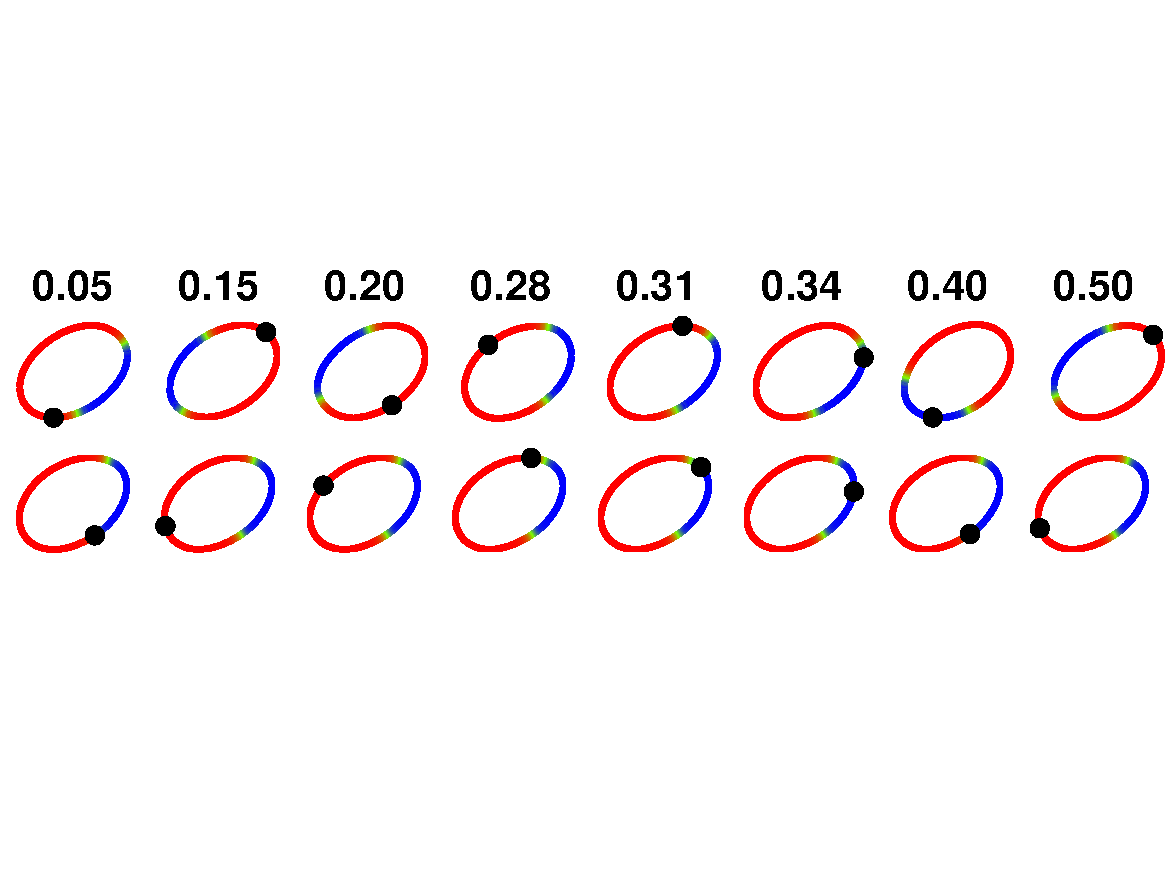
\includegraphics[width=0.9\columnwidth]{figures/shearTreading.pdf}
%  \subfigimg[width=\columnwidth, trim ={5.5cm 1.5cm 4cm 0},clip]{(a)}{figures/Fig4a.pdf}
%  \subfigimg[width=\columnwidth, trim ={5.5cm 1.5cm 4cm 0},clip]{(b)}{figures/Fig4b.pdf}
  \caption{\label{fig:treading} \small A multicomponent vesicle in a
  linear shear flow undergoes phase-treading (top) and tank-treading
  (bottom) with the new bending model~\eqref{eqn:tanhBending}. The red
  region is stiff and the blue region is floppy. The simulations
  qualitatively agree with the results presented
  by~\citet{liu-mar-li-vee-low2017}.}
\end{figure}


%\begin{figure}[h]
\begin{figure*}[h]
  \centering
  \includegraphics[width=0.9\linewidth]{figures/STENOSIS_RAp6MCp5.pdf}
%    \subfigimg[width=\columnwidth,trim ={5cm .5cm 1.5cm .5cm},clip]{(a)}{figures/Fig5a.pdf}
%    \subfigimg[width=\columnwidth,trim ={5cm .5cm 1.5cm .5cm},clip]{(b)}{figures/Fig5b.pdf}
%    \subfigimg[width=\columnwidth,trim ={5cm .5cm 1.5cm .5cm},clip]{(c)}{figures/Fig5c.pdf}
  \caption{\label{fig:RA6} \small A vesicle passing through the stenosis
  geometry. The vesicle's reduced area is $\alpha = 0.6$ and the
  capillary number is $Ca = 0.25$. The vesicles are: (a)
  single-component with bending modulus $b=1$; (b) single-component with
  bending modulus $b=0.55$; (c) multicomponent.}
%\end{figure}
\end{figure*}



%%%%%%%%%%%%%%%%%%%%%%%%%%%%%%%%%%%%%%%%%%%%%%%%%%%%%%%%%%%%%%%%%%%%%%%%
\subsection{\label{sec:LL} Lubrication layers and excess pressure}
The lubrication layer between a vesicle and the solid wall plays a
critical role on the vesicle's dynamics. Therefore, throughout
Section~\ref{sec:results}, we calculate the size and analyze the flow
inside the lubrication layers. 
%We first justify the use of the term `lubrication layer' by verifying
%that the flow velocity is parabolic between the vesicle and the solid
%wall. Figure~\ref{fig:quadraticProof} illustrates the horizontal
%velocity (solid line) and the corresponding best fit quadratic (dashed
%line) in the co-moving frame, and the profiles agree.
%
%\begin{figure}[H]
%    \centering
%    \includegraphics[width=\columnwidth]{figures/lubricationLayer_quadratic.pdf}  
%    \caption{The co-moving velocity profile in the top and bottom lubrication layers. The red curve is the velocity profile, the dashed black line is the best quadratic fit.}
%    \label{fig:quadraticProof}
%\end{figure}
To define the size of the top lubrication layer (the size of the bottom
lubrication layer is defined similarly), we let
$d(\xx,\Gamma_\mathrm{top})$ be the minimum distance between a point on
the vesicle, $\xx \in \gamma$, and the top half of the confining
geometry.
%\begin{align}
%    d(\xx,\Gamma_\mathrm{top}) = \inf_{\yy \in \Gamma_\mathrm{top}} \|\xx-\yy\|,
%\end{align}
%where $\Gamma_{\mathrm{top}}$ is the top portion of $\Gamma$.
We find all local minimums of $d(\xx,\Gamma_\mathrm{top})$, with
the condition that $d(\xx,\Gamma_\mathrm{top}) < \delta$, where $\delta$
is a parameter. If no such local minimums exist, then the vesicle is too
far from $\Gamma_\mathrm{top}$ to define a lubrication layer. If there
are two or more local minimums, the left-most, $\xx_L$, and right-most,
$\xx_R$, local minimums form the start and end of the lubrication layer.
If there is only one local minimum, then $\xx_L$ and $\xx_R$ are the
points on $\gamma$ to the left and right of this local minimum with the
condition that $d(\xx_L,\Gamma_\mathrm{top}) =
d(\xx_R,\Gamma_\mathrm{top}) = \delta$. Then, the segment
$\gamma_{\mathrm{layer}} \subset \gamma$ consists of all points $\xx \in
\gamma$ between $\xx_L$ and $\xx_R$ with the condition that
$d(\xx,\Gamma_\mathrm{top}) < \delta$. Finally, the lubrication layer
width is
\begin{align}
  w_\mathrm{top} = \frac{1}{|\gamma_{_\mathrm{layer}}|} 
    \int_{\gamma_{_\mathrm{layer}}} d(\xx,\Gamma_\mathrm{top}) \, ds.
\end{align}
The region that defines the top and bottom lubrication layers is
illustrated in Figure~\ref{fig:schematic}, and the height of the gray
regions denote the lubrication layer thickness. In this example, the top
layer is broken across three different regions.

%The terminology of boundary layer can be justified by computing the
%velocity field in the region between the vesicle and the solid wall. In
%Figure~\ref{fig:BkgrdFlow}, the co-moving velocity field around several
%different vesicle shapes that are observed in Section~\ref{sec:results}
%are illustrated. We have included plots of the horizontal velocity
%along a few vertical slices to demonstrate that a parabolic flow
%profile is observed. 

A difference between the size of the top and bottom lubrication layers
indicates that the vesicle  has deviated from the center of the channel,
and this results in tank-treading behavior~\cite{aga-bir2020}.  To
determine if a vesicle is tank-treading, we calculate the tangential
velocity at several points on $\gamma$, and if this value is constant,
this is the tank-treading velocity.

%\begin{figure}[H]
%\begin{minipage}{0.49\columnwidth}
%    \centering
%    \subfigimg[width = \columnwidth, trim = {2cm 2cm 2cm 2cm }, clip]{(a)}{figures/Fig7a1.pdf}
%    \subfigimg[width = \columnwidth, trim = {2cm 2cm 2cm 2cm }, clip]{(b)}{figures/Fig7b1.pdf}
%    \subfigimg[width = \columnwidth, trim = {2cm 2cm 2cm 2cm }, clip]{(c)}{figures/Fig7c1.pdf}
%\end{minipage}   
%\hfill
%\begin{minipage}{0.49\columnwidth}
%    \centering
%    \subfigimg[width = \columnwidth, trim = {2cm 2cm 2cm 2cm }, clip]{\color{white}(a)}{figures/Fig7a2.pdf}
%    \subfigimg[width = \columnwidth, trim = {2cm 2cm 2cm 2cm }, clip]{\color{white}(b)}{figures/Fig7b2.pdf}
%    \subfigimg[width = \columnwidth, trim = {2cm 2cm 2cm 2cm }, clip]{\color{white}(c)}{figures/Fig7c2.pdf}
%\end{minipage}
%\caption{\label{fig:BkgrdFlow} \small The velocity in the bulk, at two time steps, of a vesicle with reduced area $\alpha=0.4$. The velocity field is in the co-moving frame. The vesicles are (a) single-component with $b = 1$; (b) single-component with $b = 0.55$; and (c) multicomponent. The tangential velocity in the tubular neighborhood around the vesicle indicates that (a) and (c) are tank-treading.}    
%\end{figure}

We also report the excess pressure for one of the geometries and relate
it to the size of the lubrication layers. The excess pressure is the
additional pressure that is required to pass the vesicle through the
geometry when compared to the pressure necessary if the vesicle were
absent. These pressure calculations are taken near the inlets and
outlets of the confining geometry, and the vesicle itself is never near
these locations. Since we use a layer potential formulation, the
pressure at $\xx \in \Omega$ is
\begin{align}
  p(\xx) = \frac{1}{2\pi} \int_{\gamma} \frac{\rr \cdot \ff}{\rho^2} \, ds_\yy + 
    \frac{1}{\pi} \int_{\Gamma} \frac{1}{\rho^2} 
    \left(\mathds{I} - 2\frac{\rr \otimes \rr}{\rho^2} \right) 
    \nn \cdot \eeta \, ds_\yy.
\end{align}
%These pressure drops are defined by
%subtracting the pressure at a point near the inlet and another near the
%outlet. In our formulation, because of the order of subtraction, the
%excess pressure is always negative.


%We follow the reformulation of the governing equations outlined in Section 3.1 of \cite{soh-tse-li-voi-low2010}. In particular, we do a change of variables to the $\theta$-L formulation, where $L$ is the total length of the vesicle and $\theta$ is the opening angle of its tangent vector, $\ss$. 
%This formulation provides us with the location of a unique vesicle shape up to a translation. %, which we resolve by tracking the vesicle's center of mass. After this change of variables, the dynamics of $\theta$ are governed by
%The formulation requires the normal and tangential components of the velocity, 
%\begin{equation}
%V = \uu \cdot \nn \qquad \text{and} \qquad T = \uu \cdot \ss, \label{NormTanComp} 
%\end{equation}
%where $\nn$ is the unit normal vector and $\ss$ is the unit tangent vector. In the $\theta$-L formulation, the governing equation of the vesicle
%\begin{equation}
%\frac{d\xx}{dt} =V\nn+T\ss,
%\end{equation}
%becomes
%\begin{equation}
%\theta_t =  -(V+\beta(\textbf{f}\cdot\textbf{n}))_s + \kappa T
%\theta_t =  -V_s + \kappa T,
%\end{equation}
%and the inextensibility condition becomes
%\begin{equation}
%T_s+\kappa V  = 0. \label{genInexMC}
%\end{equation}
%Recall that the velocity $\uu$ is coupled to the tension $\sigma^{LL}$ which acts as a Lagrange multiplier to satisfy equation \eqref{genInexMC}.

%%%%%%%%%%%%%%%%%%%%%%%%%%%%%%%%%%%%%%%%%%%%%%%%%%%%%%%%%%%%%%%%%%%%%%%%
\section{\label{sec:results}Hydrodynamics of a multicomponent vesicle
under strong confinement}
We consider both a single-component and a multicomponent vesicle
suspended in two geometries: a closely-fitting geometry (stenosis) and a
geometry that slowly contracts to a narrow neck and then quickly widens
(contracting). We considered a semipermeable vesicle suspended in these
same geometries in our previous work~\cite{qua-gan-you2021}. All the
multicomponent examples have floppy-to-stiff ratio $\beta = 10^{-1}$.
For the single-component case, we consider two bending stiffnesses:
$b(u) = 1$ and $b(u) = 0.55$. % which is the average bending stiffness of a multicomponent vesicle whose stiff and floppy regions have the same area. 
The latter value represents the average bending stiffness of a multicomponent vesicle, where the stiff and floppy regions have the same area. Throughout this section we plot the position of the vesicle in terms of the $x$-coordinate of its center of mass. For the stenosed
geometry in Section~\ref{subsec:Stenosis}, the narrow region begins at
$x=-15$ and ends at $x=15$. For the contracting geometry in
Section~\ref{subsec:Contraction}, the geometry begins to narrow at $x=4$
and reaches its narrowest point at $x=15$.




%%%%%%%%%%%%%%%%%%%%%%%%%%%%%%%%%%%%%%%%%%%%%%%%%%%%%%%%%%%%%%%%%%%%%%%%

%%%%%%%%%%%%%%%%%%%%%%%%%%%%%%%%%%%%%%%%%%%%%%%%%%%%%%%%%%%%%%%%%%%%%%%%
\subsection{\label{subsec:Stenosis}A multicomponent vesicle in the
stenosis geometry}


We start by considering a vesicle with reduced area $\alpha = 0.6$
passing through stenosis with a capillary number $Ca = 0.25$.
With the current setup and $Ca=0.25$, an elliptical vesicle with reduced area greater than
$\alpha = 0.8$ cannot fit through the closely-fitting geometry.

Figure~\ref{fig:RA6} shows six time steps of a (a) stiff
single-component (b) floppy single-component, and (c) multicomponent
vesicle. The initial lipid distribution of the multicomponent vesicle is random.
In all plots, the color is the dimensionless bending modulus of the
multicomponent vesicle that remains bounded in $[0.1,1]$ by using the
new bending modulus~\eqref{eqn:tanhBending}. A single Lagrangian point
is included to visualize any tank-treading behavior. There are slight
differences between the three cases, with the most noticeable being that
the multicomponent vesicle has higher curvature in the floppy region.
However, in general, there is little difference between these cases,
partially because these vesicles have a large reduced area. 

\begin{figure*}[h]
  \centering
  \includegraphics[width=0.9\linewidth]{figures/STENOSIS_RAp4MCp5.pdf}
%    \subfigimg[width=\columnwidth,trim ={5cm .5cm 1.5cm .5cm},clip]{(a)}{figures/Fig6a.pdf}
%    \subfigimg[width=\columnwidth,trim ={5cm .5cm 1.5cm .5cm},clip]{(b)}{figures/Fig6b.pdf}
%    \subfigimg[width=\columnwidth,trim ={5cm .5cm 1.5cm .5cm},clip]{(c)}{figures/Fig6c.pdf}
  \caption{\label{fig:RA4} \small A vesicle passing through the stenosis
  geometry. The vesicle's reduced area is $\alpha = 0.4$ and the
  capillary number is $Ca = 0.25$. The vesicles are: (a) single-component
  with bending modulus $b=1$; (b) single-component with bending modulus
  $b=0.55$; (c) multicomponent.}
\end{figure*}

\begin{figure*}[ht]
  \centering
  \subfigimg[width=0.3\linewidth]{(a)}{figures/SC_energy.pdf}
  \subfigimg[width=0.3\linewidth]{(b)}{figures/SCp55_energy.pdf}
  \subfigimg[width=0.3\linewidth]{(c)}{figures/MCp5_energy.pdf}
  \caption{\label{fig:Energy} \small The bending (blue), tension (red),
  and phase (magenta) energies for a (a) stiff single-component, (b)
  floppy single-component, and (c) multicomponent vesicle. The reduced
  area is $\alpha = 0.4$. Note that the single-component vesicles do not
  have a phase energy.} 
\end{figure*}


Next we consider a vesicle with a smaller reduced area $\alpha=0.4$ with the same geometry and $Ca=0.25$.
Figure~\ref{fig:RA4} shows  the shape of  
a (a) stiff single-component, (b) floppy single-component, and (c) multicomponent
vesicle at six locations along the stenosis channel. We first consider the three different energies---bending,
tension, and phase---for each of these cases. In
Figure~\ref{fig:Energy}, we plot these energies as a function of the
vesicle's center. As a reminder, the vesicle enters the constriction at
$x=-15$ and exits at $x=15$. Also note that the single-component
vesicles do not have a phase energy. 
%A few general trends can immediately be seen. 
First we observe that, as the vesicle enters the stenosis, it
develops regions of high curvature, and this results in an increase in
the bending energy. Secondly, as the stiff single-component and
multicomponent vesicles reach a steady-state shape near the middle of
the channel, their bending, tension, and phase energies remain nearly
constant from $x=0$ until the end of the stenosis. For the multiple-component vesicle,
this implies that there is no coarsening of lipid phase in the middle of a stenosis. 

%This corresponds to an arrest of phase coarsening for a vesicle confined in a stenosis.
Such co-existence of multiple lipid domains in a vesicle under confinement
results in interesting additional physics. 
%
First we note that in Figure~\ref{fig:Energy}(c),
the lipid species coarsens at
three instances, and this results in a decrease in the phase energy.
However, as we mentioned earlier, no coarsening occurs when the vesicle is in the
closely-fitting part of the channel. Each coarsening corresponds either
to two stiff regions overtaking a small floppy region, or to two floppy
regions overtaking a small stiff region. In the first case, a region
that was originally floppy has suddenly become stiff, and this results
in a sudden increase in the bending energy. In the latter case, because
of lipid conservation, the overtaken stiff region must relocate to the
another stiff-floppy interface, and this also results in a sudden
increase in the bending energy. These increases are visible in
Figure~\ref{fig:Energy}(c) as small upticks in the blue curve. However,
in both cases, the vesicle smooths out these new regions of high
curvature, but it takes some time since the diffusion time scale is
several orders of magnitude smaller than the bending relaxation time
scale.

%\begin{figure}
%  \begin{minipage}{0.49\columnwidth}
%    \centering
%    \subfigimg[width=\textwidth]{(a)}{figures/Fig13a.pdf}
%    \subfigimg[width=\textwidth]{(c)}{figures/Fig13c.pdf}
%    \subfigimg[width=\textwidth]{(e)}{figures/Fig13e.pdf}
%  \end{minipage}
%  \hfill
%  \begin{minipage}{0.49\columnwidth}
%    \centering
%    \subfigimg[width=\textwidth]{(b)}{figures/Fig13b.pdf}
%    \subfigimg[width=\textwidth]{(d)}{figures/Fig13d.pdf}
%    \subfigimg[width=\textwidth]{(f)}{figures/Fig13f.pdf}
%  \end{minipage}
%  \caption{\label{fig:Energy} \small The Bending (blue), tension
%  (yellow), and phase (red) energies for a (a/b) single-component
%  vesicle with $b=1$, (c/d) single-component vesicle with $b = 0.55$,
%  and (e/f) multicomponent vesicle. The reduced areas are $\alpha = 0.4$
%  (a/c/e) and $\alpha = 0.6$ (b/d/f).}
%  \todo[inline]{need to redo these plots}
%\end{figure}

A main difference between the two reduced areas is that the vesicles
with smaller reduced area undergo tank-treading motions. As mentioned
earlier, tank treading occurs when the top and bottom lubrication layers
differ in size. The size of the lubrication layers for all three cases
of the vesicle with reduced area $\alpha = 0.4$ are in the top half of
Figure~\ref{fig:lubricationComposite}. Also included in the bottom of
Figure~\ref{fig:lubricationComposite} are the tank-treading velocities.
The four marker points are the Lagrangian points where the tank-treading
velocities are computed, the black dashed line is the center line of the
channel, and the rounded arrow denotes the direction of rotation. The
stiff single-component and multicomponent vesicles are clearly tank
treading. Since the single-component case has a larger difference
between its top and bottom boundary layers, it tank treads faster than
the multicomponent case. In addition, since the top boundary layer is
larger in both cases, they both tank-tread in the same
direction---counterclockwise. In contrast, the floppy single-component
vesicle tank treads in the clockwise direction; note, however, that this
example is still undergoing some deformations, so a constant
tank-treading velocity is not observed.
%When $\alpha = 0.6$, the vesicle undergoes deformations while in the
%stenosis, and a constant tank-treading velocity is not observed 


%\begin{figure}
%    \begin{minipage}{0.49\columnwidth}
%        \centering
%        \includegraphics[width=\textwidth,trim={4cm 8cm 4cm 8cm}, clip]{figures/EnergiesRAp4NoConc.pdf}
%    \end{minipage}
%    \begin{minipage}{0.49\columnwidth}
%        \centering
%        \includegraphics[width=\textwidth,trim={4cm 8cm 4cm 8cm}, clip]{figures/EnergiesRAp4Conc.pdf}
%    \end{minipage}
%    \caption{Bending (blue), tension (yellow), and phase (red) energies for a single-component vesicle %(left) and a multi-component vesicle (right) with reduced area 0.4.}
%    \label{fig:EnergyRAp4}
%\end{figure}
%\begin{figure}[H]
%    \begin{minipage}{0.49\columnwidth}
%        \centering
%        \includegraphics[width=\textwidth,trim={4cm 8cm 4cm 8cm}, clip]{figures/EnergiesRAp6NoConc.pdf}
%        \includegraphics[width=\textwidth,trim={4cm 8cm 4cm 8cm}, clip]{figures/EnergiesRAp6NoConcp55.pdf}
%    \end{minipage}
%    \hfill
%    \begin{minipage}{0.49\columnwidth}
%        \centering
%        \includegraphics[width=\textwidth,trim={4cm 8cm 4cm 8cm}, clip]{figures/EnergiesRAp6Conc.pdf}
%        \vspace{3.5cm}
%    \end{minipage}
%    \caption{Bending (blue), tension (yellow), and phase (red) energies for a single-component vesicle %(left) and a multi-component vesicle (right) with reduced area 0.6.}
%    \label{fig:EnergyRAp6l}
%\end{figure}

%\begin{figure}[h]
%    \centering
%    \subfigimg[width = 0.49\columnwidth]{(a)}{figures/Layer_Size_RAp4.pdf}
%%    \subfigimg[width = 0.49\columnwidth]{(b)}{figures/Layer_Size_RAp6.pdf}
%%    \subfigimg[width = \columnwidth]{(a)}{figures/Fig8a.pdf}\\
%%    \subfigimg[width = \columnwidth]{(b)}{figures/Fig8b.pdf}
%    \caption{\label{fig:lubrication} \small The size of the lubrication
%    layer of a stiff single-component (red), floppy single-component
%    (green), and multicomponent (blue) vesicle passing through stenosis.
%    Solid lines are the layer thickness between the vesicle and the top
%    wall, and dashed lines are the layer thickness between the vesicle
%    and the bottom wall. The reduced area of the vesicles are (a)
%    $\alpha = 0.4$ and (b) $\alpha = 0.6$.}
%\end{figure}


%Both the migration speed and tank treading behavior of a vesicle in the closely-fitting channel depends on the separation distance between the solid wall and the vesicle. As the vesicle enters the narrow constriction, lubrication layers between the vesicle and the solid walls develop. The minimum distance between the multicomponent vesicles and the solid wall (solid lines) and the single-component vesicles and the solid wall (dashed lines) are plotted in Figure~\ref{fig:lubrication}. Top top plot is for the vesicle with reduced area $\alpha = 0.4$, and the bottom plot is for the vesicle with reduced area $\alpha = 0.6$. Note that the position is only between $-15$ and $15$ which is the region with strong confinement. 

%The size of the top and bottom lubrication layers are plotted in Figure~\ref{fig:lubrication} for reduced area (a) $\alpha = 0.4$ and (b) $\alpha = 0.6$. In both cases, we see that the multicomponent vesicle has larger lubrication layers than their single-component counterparts. As shown in Figures~\ref{fig:RA6} and~\ref{fig:RA4}, the result is that the multicomponent vesicle experiences less drag from the solid walls, and therefore migrates faster. This is confirmed in Figure~\ref{fig:location1} where we plot the position of each of the vesicle versus time for both reduced areas and both lipid species. The larger lubrication layer should also result in a smaller excess pressure, especially for reduced area $\alpha = 0.4$, and this is observed in Figure~\ref{fig:excessPressure}.


%For the smaller reduced area, both the single and multicomponent vesicles are closer to the top wall than the bottom wall. More interesting, though, is that the multicomponent vesicle has a larger lubrication layer than its single-component counterpart. This larger lubrication layer means that less of the multicomponent vesicle experiences less drag from the solid wall, and its net migration speed is faster. This is verified in Figure~\ref{fig:location1}. For the larger reduced area, the vesicle is able to quickly deform away from the walls while entering the constriction. In Figure~\ref{fig:location1} we see that the multicomponent vesicle makes its way through the contstriction quicker than its single-component counterpart. Because the vesicle initially deforms, there is less initial drag from the walls. This quickly changes and the bottom lubrication layer becomes much thinner and the vesicle slows down. In Figure~\ref{fig:location1}, we can tell by the slopes of the curves that the single- and multicomponent vesicles are moving at roughly the same speed. 

%Whether a vesicle tank-treads or not is also related to the lubrication layer. In particular, if the lubrication layer between the top and lower walls are different, this indicates that the vesicle is center of mass is above or below the middle of the channel. When this happens, the non-linear of the flow results in a tank-treading vesicle.

%The smaller reduced area $\alpha = 0.4$ also results in a larger
%difference between the size of the top and boundary lubrication layers.
%In particular, Figure~\ref{fig:lubrication}(a) shows that the bottom
%lubrication layer is larger than the top lubrication layer, indicating
%the vesicle is above the centerline, and we expect the non-linear shear
%to result in a counterclockwise tank-treading motion. We define the
%tank treading velocity using several tracker points (solid points) by
%computing $\uu \cdot \tt$ where $\uu$ is the velocity and $\tt$ is the
%tangent vector at the tracker point. Note that this quantity does not
%represent a tank treading velocity until the vesicle reaches
%tank-treading behavior. Figure~\ref{fig:tankTreadRAp4} shows that for
%reduced area $\alpha = 0.4$, both the single and multicomponent
%vesicles undergo an extended period of tank-treading, but at different
%speeds, starting near the middle of the region of confinement and
%ending as the vesicles exit this region. Since the difference in sizes
%of the boundary layers is greater for the single-component vesicle, we
%expect it to tank-tread faster, which we observe when comparing
%Figures~\ref{fig:tankTreadRAp4}(a) and (e).In the multicomponent case,
%there are several interesting features in the tangential velocity, and
%these are denoted by the red marks in Figure~\ref{fig:tankTreadRAp4}.
%The vesicle shapes at each of these points are in
%Figure~\ref{fig:tankTreadRAp4}(b) and (c). The tangential velocity
%includes spikes that occur whenever there is a decrease in the phase
%energy due to floppy and stiff regions merging, and this can be
%observed in Figures~\ref{fig:tankTreadRAp4}(d) and (e). 

%\begin{figure}[h]
%    \begin{minipage}{0.49\columnwidth}
%        \centering
%        \subfigimg[width=\textwidth]{(a)}{figures/Fig11c1.pdf}
%        \subfigimg[width=\textwidth]{(c)}{figures/Fig11b1.pdf}
%        \subfigimg[width=\textwidth]{(e)}{figures/Fig11a.pdf}
%        % \subfigimg[width=\textwidth,trim={3.8cm 8cm 4cm 8cm}, clip]{(a)}{figures/TankTreadRAp4Conc.pdf}
%        % \subfigimg[width=\textwidth,trim={3.8cm 8cm 4cm 8cm}, clip]{(c)}{figures/TankTreadRANoConcp55.pdf}
%        % \subfigimg[width=\textwidth,trim={3.8cm 8cm 4cm 8cm}, clip]{(e)}{figures/TankTreadRAp4NoConc.pdf}
%        % \includegraphics[width=\textwidth,trim={3.8cm 8cm 4cm 8cm}, clip]{figures/TankTreadRAp6Conc.pdf}
%        % \includegraphics[width=\textwidth,trim={3.8cm 8cm 4cm 8cm}, clip]{figures/TankTreadRAp6NoConc.pdf}
%    \end{minipage}
%    \hfill
%    \begin{minipage}{0.49\columnwidth}
%        \centering
%        \subfigimg[width=\textwidth]{(b)}{figures/Fig11c2.pdf}
%        \subfigimg[width=\textwidth]{(d)}{figures/Fig11b2.pdf}
%        \subfigimg[width=\textwidth]{(f)}{figures/Fig11a2.pdf}
%        % \subfigimg[width=.9\textwidth,trim={4.5cm 8cm 4.5cm 8cm}, clip]{(b)}{figures/TankTreadRAp4ConcVes.pdf}
%        % \subfigimg[width=.9\textwidth,trim={4.5cm 8cm 4.5cm 8cm}, clip]{(d)}{figures/TankTreadRANoConcp55Ves.pdf}
%        % \subfigimg[width=.9\textwidth,trim={4.5cm 8cm 4.5cm 8cm}, clip]{(f)}{figures/TankTreadRAp4NoConcVes.pdf}
%        % \includegraphics[width=.9\textwidth,trim={4.5cm 8cm 4.5cm 8cm}, clip]{figures/TankTreadRAp6ConcVes.pdf}
%        % \includegraphics[width=.9\textwidth,trim={4.5cm 8cm 4.5cm 8cm}, clip]{figures/TankTreadRAp6NoConcVes.pdf}
%    \end{minipage}
%    \caption{\small The tangential velocity at four Lagrangian points on a (a) single-component vesicle with $b = 1$ (c) single-component vesicle with $b = 0.55$, and (e) multicomponent vesicle. The reduced area is $\alpha = 0.4$ in all cases. (b/d/f) A corresponding vesicle shape with the Lagrangian points.
%    \label{fig:tankTreadRAp4}}
%\end{figure}
\begin{figure*}[t]
%\begin{figure}[htp]
  \centering
  \subfigimg[width=0.3\linewidth]{(a)}{figures/Layer_Size_RAp4_SC.pdf}
  \subfigimg[width=0.3\linewidth]{(b)}{figures/Layer_Size_RAp4_SCp55.pdf}
  \subfigimg[width=0.3\linewidth]{(c)}{figures/Layer_Size_RAp4_MCp5.pdf}
  \subfigimg[width=0.3\linewidth,trim=0cm 6cm 28cm 0cm,clip=true]{}{figures/TankTreadingFigs_composite_SC.pdf}
  \subfigimg[width=0.3\linewidth,trim=0cm 6cm 28cm
  0cm,clip=true]{}{figures/TankTreadingFigs_composite_SCp55.pdf}
  \subfigimg[width=0.3\linewidth,trim=0cm 6cm 28cm
  0cm,clip=true]{}{figures/TankTreadingFigs_composite_MCp5.pdf}
  \caption{\label{fig:lubricationComposite} \small The lubrication layer
  thicknesses (red and blue), excess pressure (green), and tank treading
  velocity of four Lagrangian points of a (a) stiff single-component
  vesicle, (b) floppy single-component vesicle, and (c) multicomponent
  vesicle. The reduced area is $\alpha = 0.4$ in all three cases. Also
  illustrated is the vesicle shape and the four Lagrangian points at the
  location indicated by the dash line. The black dashed line is the
  center line of the channel, and the arrow denotes the tank treading
  direction.}
%\end{figure}
\end{figure*}


%\begin{figure}[H]
%    \begin{minipage}{0.49\columnwidth}
%        \centering
%        \subfigimg[width=\textwidth]{(a)}{figures/Fig12c1.pdf}
%        \subfigimg[width=\textwidth]{(c)}{figures/Fig12b1.pdf}
%        \subfigimg[width=\textwidth]{(e)}{figures/Fig12a1.pdf}
        % \subfigimg[width=\textwidth,trim={3.8cm 8cm 4cm 8cm}, clip]{(c)}{figures/TankTreadRAp6NoConcp55.pdf}
        % \subfigimg[width=\textwidth,trim={3.8cm 8cm 4cm 8cm}, clip]{(e)}{figures/TankTreadRAp6NoConc.pdf}
        % \includegraphics[width=\textwidth,trim={3.8cm 8cm 4cm 8cm}, clip]{figures/TankTreadRAp6Conc.pdf}
        % \includegraphics[width=\textwidth,trim={3.8cm 8cm 4cm 8cm}, clip]{figures/TankTreadRAp6NoConc.pdf}
%    \end{minipage}
%    \hfill
%    \begin{minipage}{0.49\columnwidth}
%        \centering
%        \subfigimg[width=\textwidth]{(b)}{figures/Fig12c2.pdf}
%        \subfigimg[width=\textwidth]{(d)}{figures/Fig12b2.pdf}
%        \subfigimg[width=\textwidth]{(f)}{figures/Fig12a2.pdf}
        % \subfigimg[width=.9\textwidth,trim={4.5cm 8cm 4.5cm 8cm}, clip]{(b)}{figures/TankTreadRAp6ConcVes.pdf}
        % \subfigimg[width=.9\textwidth,trim={4.5cm 8cm 4.5cm 8cm}, clip]{(d)}{figures/TankTreadRAp6NoConcp55Ves.pdf}
        % \subfigimg[width=.9\textwidth,trim={4.5cm 8cm 4.5cm 8cm}, clip]{(f)}{figures/TankTreadRAp6NoConcVes.pdf}
        % \includegraphics[width=.9\textwidth,trim={4.5cm 8cm 4.5cm 8cm}, clip]{figures/TankTreadRAp6ConcVes.pdf}
        % \includegraphics[width=.9\textwidth,trim={4.5cm 8cm 4.5cm 8cm}, clip]{figures/TankTreadRAp6NoConcVes.pdf}
%    \end{minipage}
%    \caption{\small The tangential velocity at Lagrangian points on a (a) single-component vesicle with $b = 1$ (c) single-component vesicle with $b = 0.55$, and (e) multicomponent vesicle. The reduced area is $\alpha = 0.6$ in all cases. (b/d/f) A corresponding vesicle shape with the Lagrangian points.
%    \label{fig:tankTreadRAp6}}
%\end{figure}

The size of the top and bottom lubrication layers are also related to
the excess pressure. The green curve on the top half of
Figure~\ref{fig:lubricationComposite} shows the excess pressure with the
axis aligned on the right side of the plot. When the lubrication layers
are large, most notably for the multicomponent vesicle, less pressure is
required to force the vesicle through the geometry, and the result is a
smaller (less negative) excess pressure. In contrast, when the
lubrication layers are small, most notably for the stiff
single-component vesicle, more pressure is required to force the vesicle
through the geometry, and we the result is a larger (more negative)
excess pressure.

%\begin{figure}[H]
%  \centering
%  \subfigimg[width = 0.49\columnwidth]{(a)}{figures/Excess_Pressure_RAp4}
%  \subfigimg[width = 0.49\columnwidth]{(b)}{figures/Excess_Pressure_RAp6}
%%    \subfigimg[width = 0.45\columnwidth]{(a)}{figures/Fig10a.pdf}
%%    \subfigimg[width = 0.45\columnwidth]{(b)}{figures/Fig10b.pdf}
%  \caption{\label{fig:excessPressure} \small The excess pressure a
%  stiff single-component (red), floppy single-component (green), and a
%  multicomponent (blue) vesicle moving through stenosis. The reduced
%  areas are (a) $\alpha = 0.4$, and (b) $\alpha = 0.6$.}
%\end{figure}

%While the size of the lubrication layers affect the tank-treading
%behavior and the excess pressure, it has almost no effect on the
%migration speed of the vesicle. 
%%In Figure~\ref{fig:vesVelocity}, we plot
%%the average velocity of the vesicle as it passes through the stenosed
%%region.
%With the exception of the single-component vesicle with $b=1$ and
%$\alpha = 0.6$, which has an average vesicle speed about 5\% slower, the
%average vesicle speed is constant. Obviously, this average velocity
%would be affected by the capillary number.

%\begin{figure}[H]
%  \centering
%  \includegraphics[width=\columnwidth]{figures/Fig9.pdf}
%%  \begin{tikzpicture}[scale = .6]
    \begin{axis}  
    [   axis x line = bottom,
        axis y line = left,
        xmin=0, xmax=1.1,
        xbar, bar width=10pt, 
        ylabel={}, % the ylabel must precede a # symbol.  
        xlabel={\ Vesicle velocity},  
        symbolic y coords={single-component b = 1, single-component b = 0.55, Multicomponent}, % these are the specification of coordinates on the y-axis.  
        ytick=data, 
        xticklabels={},
        xtick={},
        nodes near coords, % this command is used to mention the y-axis points on the top of the particular bar.  
        nodes near coords align={horizontal},  
        ]  
    % RA 0.4
    \addplot coordinates {(0.9402,single-component b = 1) (0.9770,single-component b = 0.55) (0.9871,Multicomponent) };  
    % RA 0.6
    \addplot coordinates {(0.9868,single-component b = 1) (0.9870,single-component b = 0.55) (0.9704,Multicomponent) }; 
\end{axis}  
\end{tikzpicture}
%  \caption{\label{fig:vesVelocity} \small The average vesicle velocity
%  as it passes through stenosis. The vesicle stiffness and reduced area
%  have no significant effect.}
%\end{figure}

When a vesicle is tank-treading near a solid wall, the flow in the thin
layer of fluid includes both a linear profile and a Poiseuille
profile~\cite{mis-wis-ber-key-li-tun-law-per-erd-zha-zha-sun-kal-lam-kon2019}.
The magnitude of the Poiseuille profile is determined by the pressure
gradient between the vesicle and the solid wall, while the linear
profile is determined by the tangential velocity of the vesicle relative
to the solid wall. Using the definition of the lubrication layer
outlined in Section~\ref{sec:LL}, we consider the flow profile inside
this lubrication layer in Figure~\ref{fig:BLvelocities}. We observe that
the Poiseuille coefficient can be either positive or negative, meaning
that the pressure in the lubrication layer switches signs. This behavior
is caused when the tangential force on the vesicle
\begin{align}
  \mathbf{F}_{\tt} = -\sigma_s + u_s \frac{\delta E^m}{\delta u},
\end{align}
switches sign. Here,
\begin{align}
  \frac{\delta E^m}{\delta u} = \frac{a}{\epsilon} 
    (f'(u) - \epsilon^2 u_{ss}) + \frac{b'(u)}{2} \kappa^2
\end{align}
is the variational derivative of the membrane energy with respect to the
lipid concentration~\cite{soh-tse-li-voi-low2010}. Note that in the
single-component case, the tangential force is $\mathbf{F}_\tt =
-\sigma_s$ which is the usual Marangoni effect.

\begin{figure*}[t]
%\begin{figure}
  \centering
  \subfigimg[width=0.48\linewidth]{(a)}{figures/SC_top.pdf}
  \subfigimg[width=0.48\linewidth]{(b)}{figures/SC_bot.pdf}
  \subfigimg[width=0.48\linewidth]{(c)}{figures/SCp55_top.pdf}
  \subfigimg[width=0.48\linewidth]{(d)}{figures/SCp55_bot.pdf}
  \subfigimg[width=0.48\linewidth]{(e)}{figures/MCp5_top.pdf}
  \subfigimg[width=0.48\linewidth]{(f)}{figures/MCp5_bot.pdf}
  \caption{\label{fig:BLvelocities} \small The co-moving velocity field
  in the thin fluid layer between vesicles and the stenosis geometry.
  The vesicles are (a/b): single-component with $b(u) = 1$; (c/d):
  single-component with $b(u) = 0.55$; (e/f): multicomponent. The top
  layers are in (a/c/e) and the bottom layers are in (b/d/f). The
  profiles are ploted at slices where the pressure gradient transitions
  from a value that is negative, zero, positive, zero, and negative. The
  right plots show the tangential stress with the five slices denoted by
  the marks. Note that the reversal in the pressure gradient occurs when
  the tangential stress is sufficiently large, in magnitude.}
%\end{figure}
\end{figure*}


%%%%%%%%%%%%%%%%%%%%%%%%%%%%%%%%%%%%%%%%%%%%%%%%%%%%%%%%%%%%%%%%%%%%%%%%
\subsection{\label{subsec:Contraction} A multicomponent vesicle in the
contracting geometry}
In this section, we consider a single vesicle passing through a geometry
that slowly contracts to a region that is only 2~$\mu$m wide, and then
immediately opens back up to a channel that is ten times larger. We
first consider the effect of the initial lipid concentration when the
floppy and stiff regions each make up half of the vesicle membrane. In
Figure~\ref{fig:RA6leftRightRand}, snapshots of vesicles with reduced
area $\alpha = 0.6$ with different initial lipid distributions are
illustrated. The initial distributions are random (middle) floppy in the
front and stiff in the back (top), and one that is stiff in the front
and floppy in the back (bottom). The vesicle with the random initial
lipid distribution quickly phase separates into two floppy and two stiff
regions. As seen in the stenosis geometry, further phase separation is
delayed until the vesicle is no longer under strong confinement. The
vesicle with the floppy region on the front reorients the floppy region
towards the back of the vesicle. In contrast, the vesicle with the stiff
region at the front maintains its orientation. In summary, in all three
cases, the vesicle is orienting itself so that the stiff region passes
through the constriction before the floppy region.  Therefore, in
subsequent simulations, we initialize the vesicle's lipid concentration
so that the floppy region is in the back and its stiff region is in the
front. The vesicle shapes develop regions with high curvature in the
floppy region when they first pass through the narrowest part of the
geometry, but because the strong confinement is abruptly removed
immediately afterwards, these regions of high curvature are quickly
smoothed. 
%Since we can see in Figure~\ref{fig:RA6leftRightRand} that the regions
%of high curvature are located in the back of the vesicle, we expect the
%overall bending energies to be lowest for the randomly distributed case
%and the fully separated floppy region on the back case. We observe this
%in Figure~\ref{fig:RAp6leftRightRandBending}. 

\begin{figure}[h]
  \centering
%    \subfigimg[width=\columnwidth,trim ={5cm .5cm 2cm .5cm},clip]{(a)}{figures/rightSep.pdf}
%    \subfigimg[width=\columnwidth,trim ={5cm .5cm 2cm .5cm},clip]{(b)}{figures/randSep.pdf}
%    \subfigimg[width=\columnwidth,trim ={5cm .5cm 2cm .5cm},clip]{(c)}{figures/leftSep.pdf}
  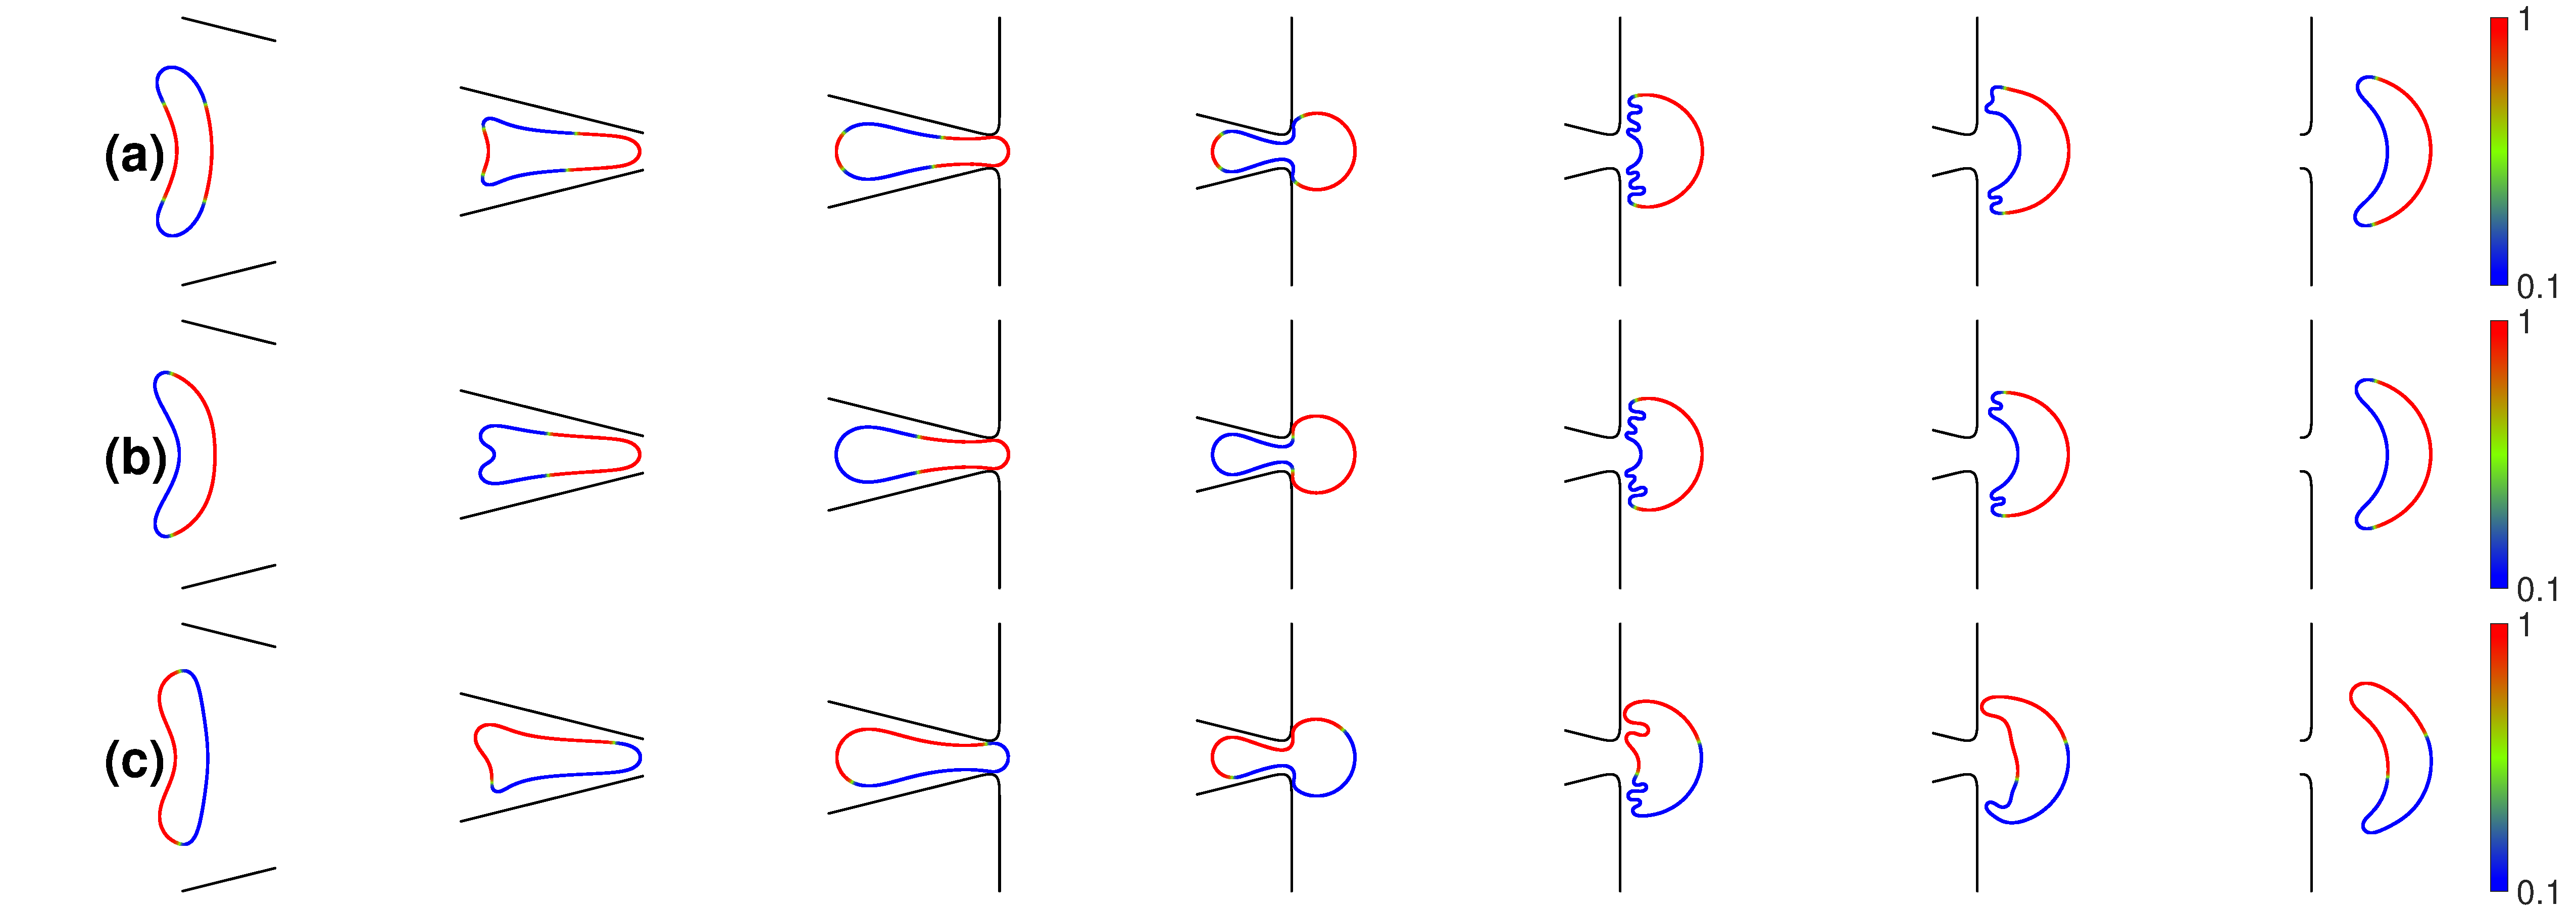
\includegraphics[width=\columnwidth]{figures/Contracting_RAp6MCp5.pdf}
  \caption{\label{fig:RA6leftRightRand} \small A multicomponent vesicle
  with 50\% floppy region passing through a contracting geometry. The
  vesicle's reduced area is $\alpha = 0.6$ and the capillary number is
  $Ca = 0.25$. The lipid distribution is initialized to be (a) phase
  separated with the floppy region leading; (b) random; (c) phase
  separated with the stiff region leading.}
\end{figure}

%\begin{figure}[H]
%  \centering
%  \includegraphics[width=\columnwidth]{figures/bending_leftRightRand.pdf}
%  \caption{\label{fig:RAp6leftRightRandBending} The bending energy of a
%  multicomponent vesicle that is 50\% stiff with an initial phase
%  separation to the left (blue), to the right (red), randomly
%  distributed (yellow). The vesicle exits the contraction $x \approx
%  15$.} 
%\end{figure}

In addition to the lipid distribution, the percentage of the vesicle
that is floppy plays a role in the vesicle shapes and dynamics.
Therefore, we consider a vesicle with reduced area $\alpha = 0.5$ in the
contracting geometry with various sizes of the floppy region. Motivated
by the last experiment, we initialize the stiff region to be in the
front and the floppy region to be in the back. In each simulation, the
capillary number is $Ca = 0.25$. Figure~\ref{fig:RA5} shows the vesicle
shapes at the same six time steps when the percentage of the floppy
region is 0\% (single-component), \%15, \%25, \%35, and \%45. One effect
of the size of the floppy region is that the symmetry of the vesicle
shape is broken at smaller percentages. We also see that stiffer
vesicles have faster migration speeds, but the effect is quite
small---Table~\ref{tbl:contractingTimes} reports the time the vesicle
first passes through the neck.
%In Figure~\ref{fig:RA5}, we consider a vesicle with reduced area
%$\alpha = 0.5$ and the capillary number is $Ca = 0.25$. We start with a
%single-component vesicle and then increase the percentage of the
%vesicle membrane that is floppy. By comparing the vesicle location at
%the time step just before the vesicle passes through the constriction,
%we can immediately see that vesicles with membranes that have larger
%percentage of floppy regions reach and pass through the neck earlier.
%The dimensionless times that the entire vesicle first passes through
%the neck are reported in Table~\ref{tbl:contractingTimes}.

%\begin{figure*}[t]
\begin{figure}[h]
  \centering
  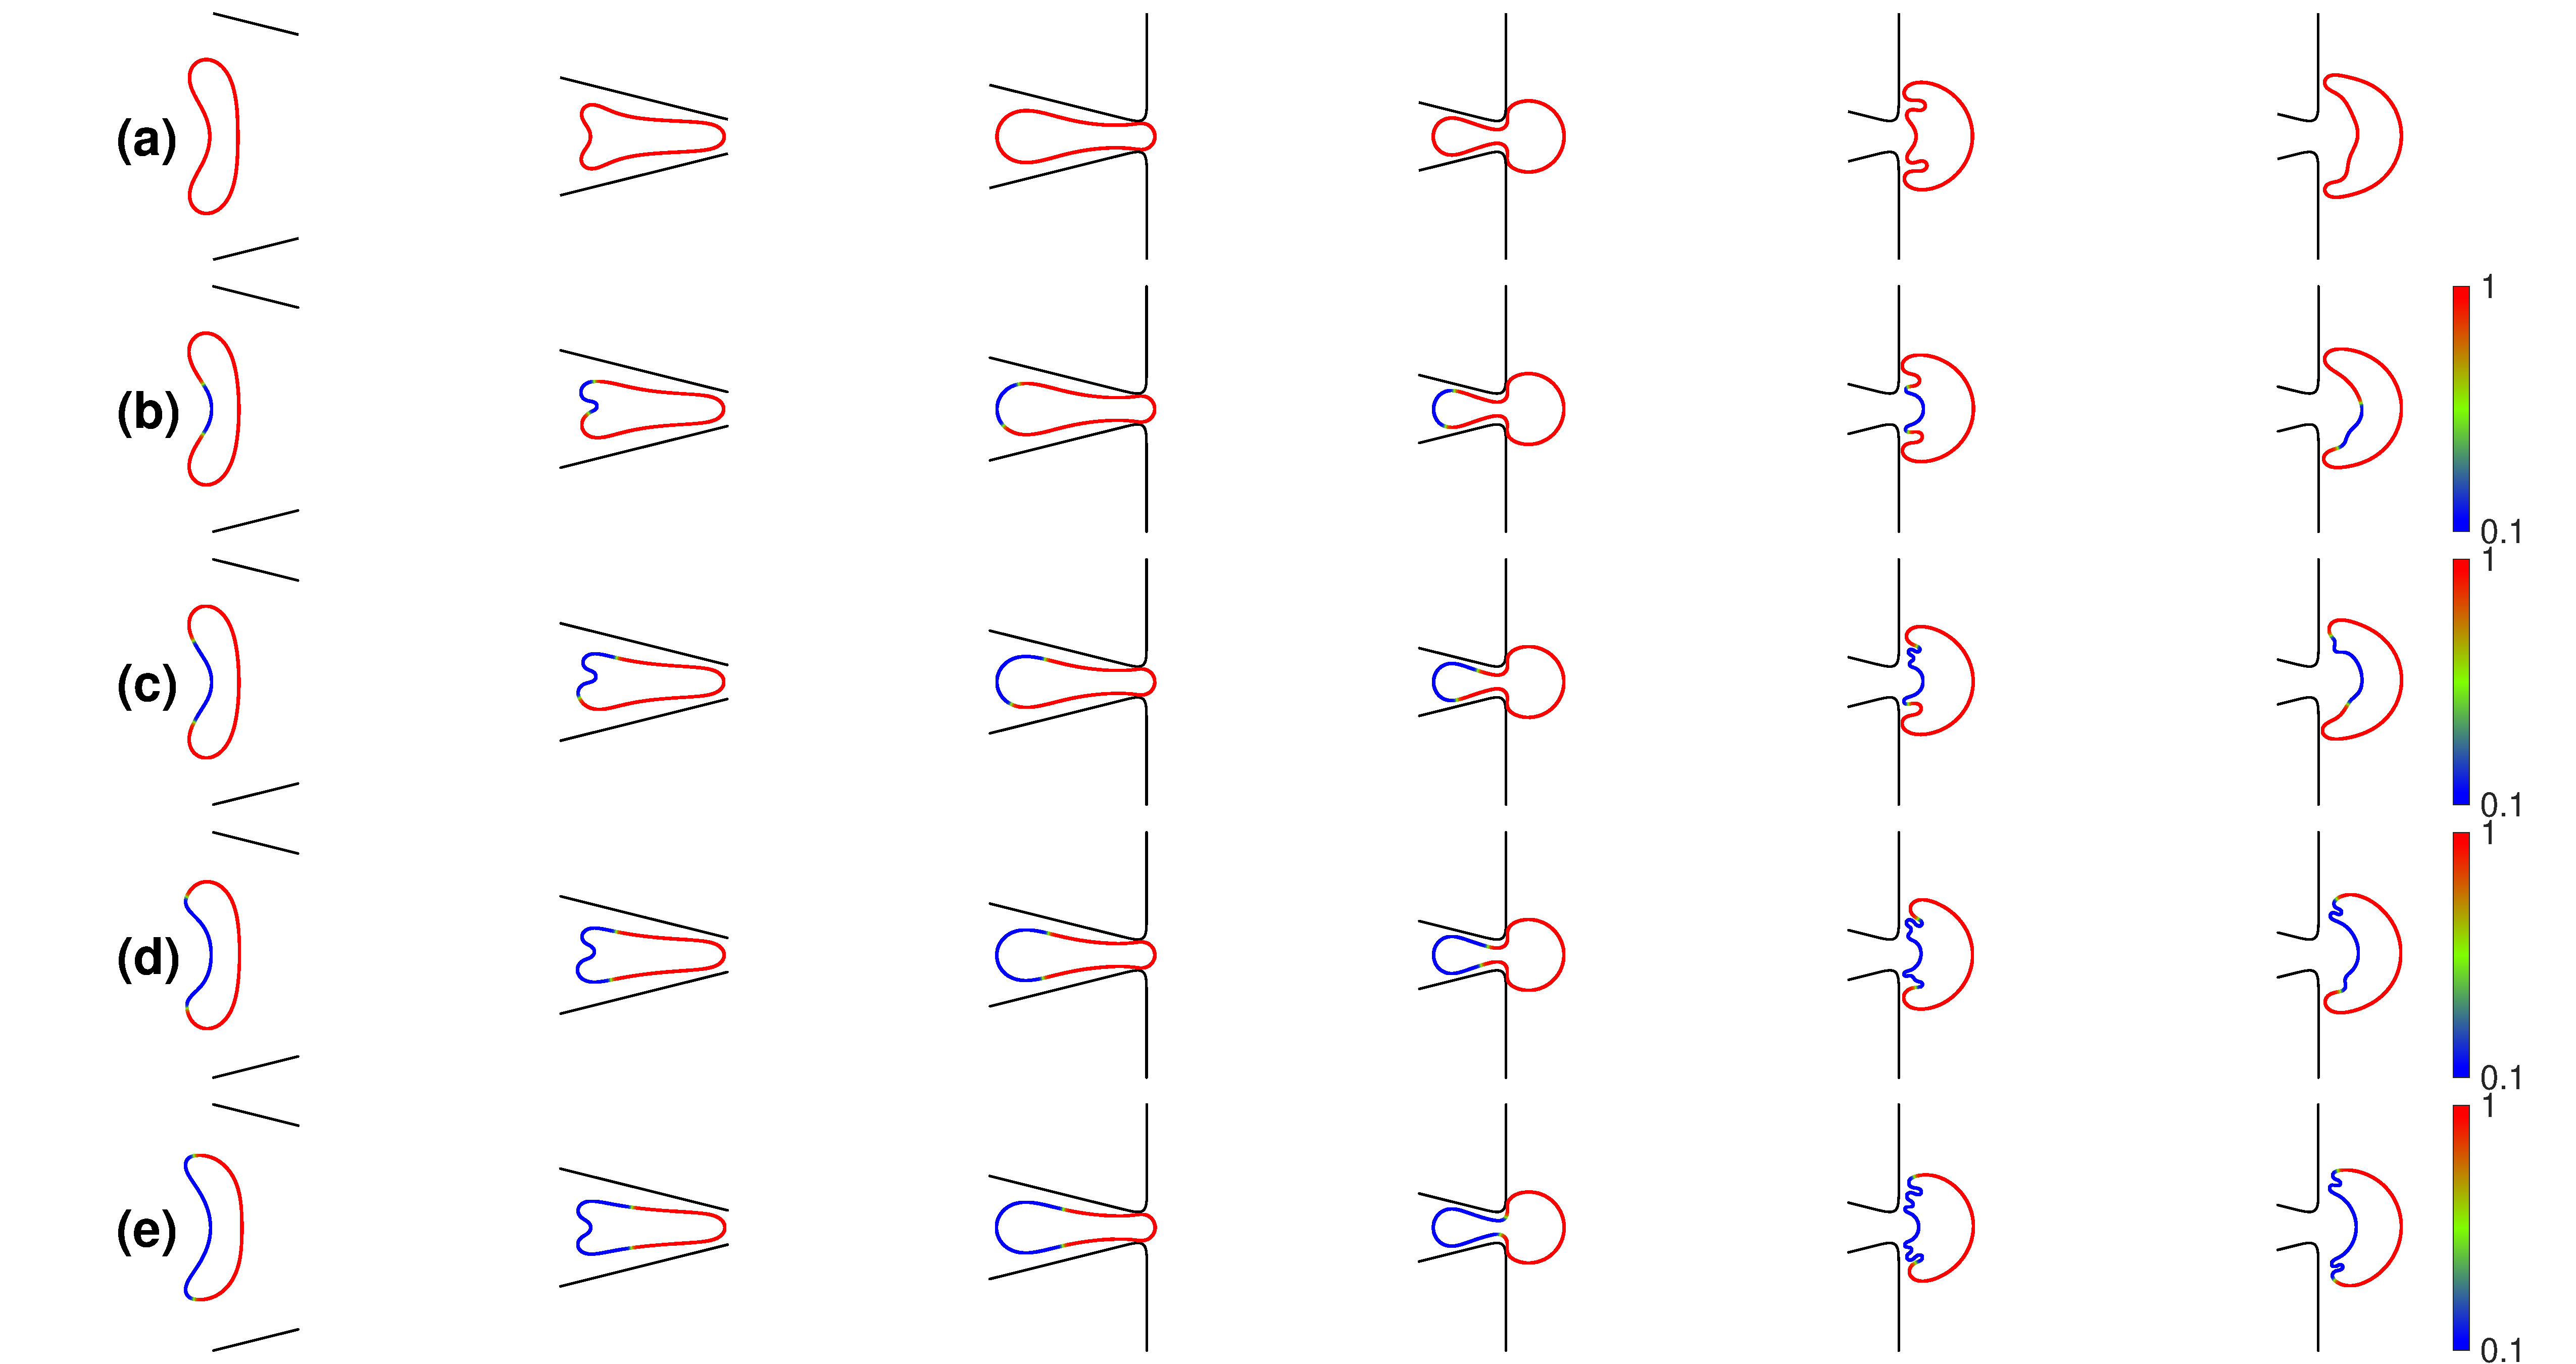
\includegraphics[width=\columnwidth]{figures/Contracting_RAp6MC_variableConc.pdf}
%    \subfigimg[width=\columnwidth,trim ={5cm .5cm 1.5cm .5cm},clip]{(a)}{figures/Fig14f.pdf}
%    \subfigimg[width=\columnwidth,trim ={5cm .5cm 1.5cm .5cm},clip]{(b)}{figures/Fig14a_newPaper.pdf}
%    \subfigimg[width=\columnwidth,trim ={5cm .5cm 1.5cm .5cm},clip]{(c)}{figures/Fig14b_newPaper.pdf}
%    \subfigimg[width=\columnwidth,trim ={5cm .5cm 1.5cm .5cm},clip]{(d)}{figures/Fig14c_newPaper.pdf}
%    \subfigimg[width=\columnwidth,trim ={5cm .5cm 1.5cm .5cm},clip]{(e)}{figures/Fig14e_newPaper.pdf}
  \caption{\label{fig:RA5} \small A vesicle passing through a
  contracting geometry. The vesicle's reduced area is $\alpha = 0.5$ and
  the Capillary number is $Ca = 0.25$. The vesicles are: (a)
  single-component with bending modulus $b=b_{\max}$; (b) multicomponent
  with 15\% floppy region; (c) multicomponent with 25\% floppy region;
  (d) multicomponent with 35\% floppy region; (e) multicomponent with
  45\% floppy region. The vesicles with a larger percentage of floppy
  regions pass through the neck earlier than the vesicles with less
  percentage of floppy regions.}
\end{figure}
%\end{figure*}

\begin{table}[h]
  \centering
  \begin{tabular}{l|ccccc}
    \hline
    Floppy percentage & 0\% & 15\% & 25\% & 35\% & 45\% \\ 
    Time  & 2.32 & 2.30 & 2.29 & 2.26 & 2.24 \\
    \hline
  \end{tabular}
  \caption{\label{tbl:contractingTimes} \small The time required for the
  vesicles to completely pass through the neck.}
\end{table}
%\begin{table}[H]
%  \centering
%  \begin{tabular}{l|c}
%    Floppy percentage & Time to pass through neck \\
%    \hline
%    0\% &  2.32 \\
%    15\% & 2.30 \\
%    25\% & 2.29 \\
%    35\% & 2.26 \\
%    45\% & 2.24 \\
%%    Single-component &  2.32 \\ %2.3173\\
%%    15\% Multicomponent & 2.30 \\%2.2960\\
%%    25\% Multicomponent & 2.29 \\%2.2868\\
%%    35\% Multicomponent & 2.26 \\%2.2637\\
%%    45\% Multicomponent & 2.24 \\%2.2388\\
%    \hline
%  \end{tabular}
%  \caption{\label{tbl:contractingTimes} The time required for the
%  vesicles to completely pass through the neck.}
%\end{table}

\begin{figure}[h]
  \centering
  \includegraphics[width=\columnwidth]{figures/bendingContracting.pdf}
%  \includegraphics[width=\columnwidth]{figures/bendingAllContracting.pdf}
  \caption{\label{fig:bendingAll} \small The bending energy for a
  single-component vesicle (blue) and a multicomponent vesicle
  (red)--(black) with $\alpha = 0.5$. As the size of the floppy region
  increases, the maximum bending energy decreases.}
\end{figure}

We conclude this example by considering the different shapes that
single-component and multicomponent shapes display. Since we have
initialized the lipid species to initially be phase separated, the phase
energy is nearly constant for all cases, and is therefore not plotted.
The tension energy, on the other hand, increases as the vesicle
approaches the neck, but its general shape is similar for all five
cases, and it too is not plotted. However, the bending energies show
different behaviors for each of the cases (Figure~\ref{fig:bendingAll}).
The main difference being that the multicomponent vesicles with a higher
percentage of floppy regions have less bending energy, especially as the
vesicle passes through the neck. We also note that the bending energy
undergoes several transient increases and decreases. These occur when
the tail of the vesicle undergoes transitions from lower energy shapes,
such as `C' or `S' shapes, to high energy shapes, such as 'W' shapes.
Figure~\ref{fig:bendingSC_contracting} shows these different vesicle
shapes for the single-component vesicle and multicomponent vesicle that
is 45\% floppy. The shapes at several critical points along the bending
energy are included, and we can indeed see that transitioning vesicle
shape between these different states.

\begin{figure}[h]
  \centering
%    \subfigimg[width=\columnwidth,trim ={5cm .5cm 1.5cm .5cm},clip]{(a)}{figures/Fig14f.pdf}
  \subfigimg[width=\columnwidth]{(a)}{figures/ContractingEnergy_SC.pdf}
  \subfigimg[width=\columnwidth]{(b)}{figures/ContractingEnergy_MC.pdf}
%  \subfigimg[width=\columnwidth]{(a)}{figures/bendingSC.pdf}
%  \subfigimg[width=\columnwidth]{(b)}{figures/bendingEngMC45.pdf}
  \caption{\label{fig:bendingSC_contracting} \small The bending energy
  of (a) a single-component vesicle, and (b) a multicomponent vesicle
  whose boundary is 45\% floppy passing through a contracting geometry.
  The vesicle shape at different locations are included. We can clearly
  see that the sudden increases and decreases in the bending energy are
  due to transitions between lower energy and higher energy shapes.}
\end{figure}



%\begin{figure}
%  \begin{minipage}{0.49\columnwidth}
%    \centering
%    \subfigimg[width=\textwidth]{(a)}{figures/Fig15i.pdf}
%    \subfigimg[width=\textwidth]{(c)}{figures/Fig15a.pdf}
%    \subfigimg[width=\textwidth]{(e)}{figures/Fig15c.pdf}
%    \subfigimg[width=\textwidth]{(g)}{figures/Fig15e.pdf}
%    \subfigimg[width=\textwidth]{(i)}{figures/Fig15g.pdf}
%  \end{minipage}
%  \hfill
%  \begin{minipage}{0.49\columnwidth}
%    \centering
%    \subfigimg[width=\textwidth]{(b)}{figures/Fig15j.pdf}
%    \subfigimg[width=\textwidth]{(d)}{figures/Fig15b.pdf}
%    \subfigimg[width=\textwidth]{(f)}{figures/Fig15d.pdf}
%    \subfigimg[width=\textwidth]{(h)}{figures/Fig15f.pdf}
%    \subfigimg[width=\textwidth]{(j)}{figures/Fig15h.pdf}
%  \end{minipage}
%  \caption{\label{fig:Energy} \small The bending (blue), tension (yellow), and phase (red) energies for a single-component vesicle ((a) and (b)) and a multicomponent vesicle (c)--(j) with $\alpha = 0.5$. As the size of the floppy region increases, the maximum bending energy decreases.}
%\end{figure}

%\begin{itemize}
%    \item Look at single-component vs. multicomponent with two different reduced areas and using random and non-random initial lipid distributions
%    \begin{itemize}
%        \item Show the floppy region rotating around to/forming in the back
%        \item \todo[inline]{$\Chi = 0.5 \mu$m/s, RA = 0.4, single component, multi component (random, left, right)}
%        \item \todo[inline]{$\Chi = 0.5 \mu$m/s, RA = 0.6 (for consistency, BUT maybe just the RA = 0.5 is sufficient since they all also do not make it), single component, multi component (random, left, right)}
%        \item \todo[inline]{Look at the $\Chi = 5 \mu$m/s runs to see how these compare. Idea - Slower runs allow more time for the floppy region to move around.} 
%        \item The RA = 0.4 cases all move through the contraction for both flow rates. All the RA = 0.5 cases get stuck for both flow rates.
%    \end{itemize}
%    \begin{figure}[H]
%        \centering
%        \subfigimg[width=\columnwidth,trim ={5cm .5cm 1.5cm .5cm},clip]{(a)}{figures/Fig14f.pdf}
%       \subfigimg[width=\columnwidth,trim ={5cm .5cm 1.5cm .5cm},clip]{(b)}{figures/Fig14a.pdf}
%        \subfigimg[width=\columnwidth,trim ={5cm .5cm 1.5cm .5cm},clip]{(c)}{figures/Fig14b.pdf}
        %\subfigimg[width=\columnwidth,trim ={5cm .5cm 1.5cm .5cm},clip]{(d)}{figures/Fig14d.pdf}
%        \subfigimg[width=\columnwidth,trim ={5cm .5cm 1.5cm .5cm},clip]{(d)}{figures/Fig14c.pdf}
%        \subfigimg[width=\columnwidth,trim ={5cm .5cm 1.5cm .5cm},clip]{(e)}{figures/Fig14e.pdf}
%        \caption{\label{fig:RA5} \small Snapshots of a vesicle passing through a contracting geometry. In all cases, the vesicle's reduced area is $\alpha = 0.5$ and the dimensionless maximum velocity is $\chi = 0.25$. The vesicles are: (a) single-component with bending modulus $b=1$; (b) Multicomponent with 15\% floppy region; (c) Multicomponent with 25\% floppy region; (d) Multicomponent with 35\% floppy region; (e) Multicomponent with 45\% floppy region. We see that the vesicles with a larger percentage of floppy regions pass through the neck earlier than the vesicles with less percentage of floppy regions.}
        %\caption{\label{fig:RA6} A single-component (top) and multicomponent (bottom) vesicle passing through the stenosed geometry. In both simulations, the reduced area is $0.6$ and the dimensionless maximum velocity is $\chi = 0.25$. Note that the multicomponent vesicle travels slightly faster, so it leaves the narrow constriction earlier (see Figure~\ref{fig:location1}.}
%    \end{figure}

%    \begin{figure}
%      \begin{minipage}{0.49\columnwidth}
%        \centering
%    %    \subfigimg[width = \columnwidth, trim = {1cm 20cm 1cm 3cm}, clip]{(a)}{figures/RAp4BkgrdFlow.pdf}
%        \subfigimg[width=\textwidth]{(a)}{figures/Fig15i.pdf}
%        \subfigimg[width=\textwidth]{(c)}{figures/Fig15a.pdf}
%        \subfigimg[width=\textwidth]{(e)}{figures/Fig15c.pdf}
%        \subfigimg[width=\textwidth]{(g)}{figures/Fig15e.pdf}
%        \subfigimg[width=\textwidth]{(i)}{figures/Fig15g.pdf}
%        
%      \end{minipage}
%      \hfill
%      \begin{minipage}{0.49\columnwidth}
%        \centering
%        \subfigimg[width=\textwidth]{(b)}{figures/Fig15j.pdf}
%        \subfigimg[width=\textwidth]{(d)}{figures/Fig15b.pdf}
%        \subfigimg[width=\textwidth]{(f)}{figures/Fig15d.pdf}
%        \subfigimg[width=\textwidth]{(h)}{figures/Fig15f.pdf}
%        \subfigimg[width=\textwidth]{(i)}{figures/Fig15h.pdf}
        
%      \end{minipage}
%      \caption{\label{fig:Energy} \small The Bending (blue), tension (yellow), and phase (red) energies for a (a/b/c/d/e/f/g/h) Multicomponent vesicle, (i/j) single-component vesicle with $\alpha = 0.5$. As the size of the floppy region increases, the maximum bending energy decreases.}
%    \end{figure}

    
%    \item Vesicle has a `preferred orientation' - forces the floppy region to the back. The question becomes: Is there a Goldilocks region where there is enough floppy region in the back for the vesicle to pass through? (RA = 0.5)
%    \begin{itemize}
%        \item \todo[inline]{$Chi = 5 \mu$m/s, 10\% floppy}
%        \item \todo[inline]{$Chi = 5 \mu$m/s, 30\% floppy}
%        \item \todo[inline]{$Chi = 5 \mu$m/s, 50\% floppy}
%        \item \todo[inline]{$Chi = 5 \mu$m/s, 90\% floppy}
%    \end{itemize}
%    \item Investigate why the 30\% case makes it though. Hopefully there's a story in these plots:
%    \begin{itemize}
%        \item \todo[inline]{Excess pressure plots of all}
%        \item \todo[inline]{Boundary layer plots of all}
%        \item \todo[inline]{Energy plots of all}
%        \item W, S, to C. (something to explore, floppy/stiff regions bending energy)
%    \end{itemize}
    
%    \item Discuss the shapes of the vesicles after they pass through the contraction. Lots of oscillations in the floppy region
%    \begin{itemize}
%        \item Maybe include error plots or a maximum error. 
%    \end{itemize}
%\end{itemize}




\section{Conclusions \label{sec:conclusion}}
In this work we used numerical simulations to examine the hydrodynamics of a multicomponent vesicle under strong confinement, which is a ubiquitous configuration in biology when a cell squeezes through a small channel. We refined the phase-field formulation in \citet{liu-mar-li-vee-low2017} with a new bending model that uses a sigmoidal function for the bending stiffness to retain positiveness in the bending modulus. The linear model \cite{liu-mar-li-vee-low2017} works well for a vesicle in free-space. However, under strong confinement we find it necessary to enforce the condition that the dimensionless bending modulus $b(u)$ be in the range of $[\beta,1]$  ($\beta = b_{\min}/b_{\max}$)  to avoid instability in membrane shapes (see \S~\ref{subsec:const_eq}). We focused on the hydrodynamics of a multicomponent vesicle in two types of confinement: a stenosis channel (\S~\ref{subsec:Stenosis}), and a contracting channel (\S~\ref{subsec:Contraction}). For both confining geometries we varied the reduced area $\alpha$, the floppy-to-stiffness ratio $\beta$, and the initial distribution of lipid domains with a fixed Capillary number $Ca=0.25$ and a fixed Peclet number of the lipid dynamics $Pe=1$.  In \S~\ref{subsec:Stenosis} the confinement ratio (defined as $2R_0/W$) in the stenosis is $1.67$, and in \S~\ref{subsec:Contraction} the confinement ratio increases to a maximum of $2$ at the neck. Consequently the dependence of the vesicle shape on the capillary number is expected to be less sensitive according to results in \citet{aga-bir2020}. Finally the phase separation is assumed to occur at a much faster time scale than vesicle relaxation with Pectlet number $Pe=1$.

As a multicomponent vesicle enters/leaves a closely-fitted stenosis, coarsening of the lipid domains is expedited. However, inside the stenosis, the strong confinement hinders the coarsening as both the vesicle shape and the lipid domains remain more or less un-altered as the vesicle moves through the stenosis. Once inside a stenosis, we define the lubrication layer and its corresponding width to analyze the mechanical coupling between the boundaries in lipid domain and the planar shear flow inside the lubrication layer, which consists of a quadratic component (due to pressure gradient in the thin film) and a linear component (due to membrane motion in the tangential direction). By analyzing these two components at various locations in the lubrication layer, we first identified that tank treading along the vesicle of $\alpha=0.4$ is due to the mismatch in lubrication layer width on the two sides.  We further elucidated  the correlation between the location of boundary between lipid domains, the Marangoni stress,  and the change of sign in the pressure gradient in the lubrication layer. These results may be used to identify the lipid domains via the visualization of the flow in the lubrication layer.

For a multicomponent vesicle squeezing through a constriction, we simulated the passage of a vesicle with various initial configurations of lipid domains. We found that, once the vesicle makes its passage, the front of the vesicle is often stiffer than the back of the vesicle, with a similar shape of a smaller curvature in the front than the curvature in the back. This is also observed for a vesicle moving out of confinement from a stenosis channel. Thus we propose a strong confinement in combination with a sharp transition to a wider opening can be used to produce phase-separated multicomponent vesicle with the floppy lipid species in the back and the stiff lipid species in the front of the vesicle.

Such asymmetry in lipid domain induced by strong confinement and sudden release gives rise to a nonuniform tension distribution in the membrane, with higher (?) tension in the front and lower (?) tension in the back. This may have biophysical consequences in polarity developing of a migrating cell.


%\begin{itemize}
%  \item New bending model using hyperbolic tangent (sigmoidal shape)
%    which is necessary to maintain a positive bending modulus
%
%  \item Orientation of the phase is always stiff on the front and floppy
%    on the back, but we don't know why (yet). Observed by others such as
%    Biros and Agrawalla, George and Misbah, and others.
%
%  \item Boundary layer and change in sign of pressure gradient term that
%    drives the lubrication flow. This is a combination of the tension
%    and the phase boundary between stiff and floppy regions.
%
%  \item Sudden drop in bending energy for multicomponent can be
%    explained by the sudden coarsening of the lipids.
%
%  \item Relationship between tank treading, excess pressure and layer
%    thickness.
%
%  \item  Inability to coarsen when under strong confinement. Can be
%    related to item 2. Strong confinement arrests phase coarsening.
%
%\end{itemize}

%The main text of the article\cite{Mena2000} should appear here.
%
%\subsection{This is the subsection heading style}
%Section headings can be typeset with and without numbers.\cite{Abernethy2003}
%
%\subsubsection{This is the subsubsection style.~~} These headings should end in a full point.  
%
%\paragraph{This is the next level heading.~~} For this level please use \texttt{\textbackslash paragraph}. These headings should also end in a full point.
%
%\section{Graphics and tables}
%\subsection{Graphics}
%Graphics should be inserted on the page where they are first mentioned (unless they are equations, which appear in the flow of the text).\cite{Cotton1999}
%
%\begin{figure}[h]
%\centering
%  \includegraphics[height=3cm]{example1}
%  \caption{An example figure caption \textendash\ the image is from the \textit{Soft Matter} cover gallery.}
%  \label{fgr:example}
%\end{figure}
%
%\begin{figure*}
% \centering
% \includegraphics[height=3cm]{example2}
% \caption{An image from the \textit{Soft Matter} cover gallery, set as a two-column figure.}
% \label{fgr:example2col}
%\end{figure*}
%
%\subsection{Tables}
%Tables typeset in RSC house style do not include vertical lines. Table footnote symbols are lower-case italic letters and are typeset at the bottom of the table. Table captions do not end in a full point.\cite{Arduengo1992,Eisenstein2005}
%
%
%\begin{table}[h]
%\small
%  \caption{\ An example of a caption to accompany a table}
%  \label{tbl:example1}
%  \begin{tabular*}{0.48\textwidth}{@{\extracolsep{\fill}}lll}
%    \hline
%    Header one (units) & Header two & Header three \\
%    \hline
%    1 & 2 & 3 \\
%    4 & 5 & 6 \\
%    7 & 8 & 9 \\
%    10 & 11 & 12 \\
%    \hline
%  \end{tabular*}
%\end{table}
%
%Adding notes to tables can be complicated.  Perhaps the easiest method is to generate these manually.\footnote[4]{Footnotes should appear here. These might include comments relevant to but not central to the matter under discussion, limited experimental and spectral data, and crystallographic data.}
%
%\begin{table*}
%\small
%  \caption{\ An example of a caption to accompany a table \textendash\ table captions do not end in a full point}
%  \label{tbl:example2}
%  \begin{tabular*}{\textwidth}{@{\extracolsep{\fill}}lllllll}
%    \hline
%    Header one & Header two & Header three & Header four & Header five & Header six  & Header seven\\
%    \hline
%    1 & 2 & 3 & 4 & 5 & 6  & 7\\
%    8 & 9 & 10 & 11 & 12 & 13 & 14 \\
%    15 & 16 & 17 & 18 & 19 & 20 & 21\\
%    \hline
%  \end{tabular*}
%\end{table*}
%
%\section{Equations}
%
%Equations can be typeset inline \textit{e.g.}\ $ y = mx + c$ or displayed with and without numbers:
%
% \[ A = \pi r^2 \]
%
%\begin{equation}
%  \frac{\gamma}{\epsilon x} r^2 = 2r
%\end{equation}
%
%You can also put lists into the text. You can have bulleted or numbered lists of almost any kind. 
%The \texttt{mhchem} package can also be used so that formulae are easy to input: \texttt{\textbackslash ce\{H2SO4\}} gives \ce{H2SO4}. 
%
%For footnotes in the main text of the article please number the footnotes to avoid duplicate symbols. \textit{e.g.}\ \texttt{\textbackslash footnote[num]\{your text\}}. The corresponding author $\ast$ counts as footnote 1, ESI as footnote 2, \textit{e.g.}\ if there is no ESI, please start at [num]=[2], if ESI is cited in the title please start at [num]=[3] \textit{etc.} Please also cite the ESI within the main body of the text using \dag. For the reference section, the style file \texttt{rsc.bst} can be used to generate the correct reference style.
%
%\section{Conclusions}
%The conclusions section should come in this section at the end of the article, before the Conflicts of interest statement.
%
%
%\section*{Author Contributions}
%We strongly encourage authors to include author contributions and recommend using \href{https://casrai.org/credit/}{CRediT} for standardised contribution descriptions. Please refer to our general \href{https://www.rsc.org/journals-books-databases/journal-authors-reviewers/author-responsibilities/}{author guidelines} for more information about authorship.

\section*{Conflicts of interest}
There are no conflicts to declare.

\section*{Acknowledgements}
The Acknowledgements come at the end of an article after Conflicts of interest and before the Notes and references.

%%%END OF MAIN TEXT%%%

%The \balance command can be used to balance the columns on the final page if desired. It should be placed anywhere within the first column of the last page.

\balance

%If notes are included in your references you can change the title from 'References' to 'Notes and references' using the following command:
%\renewcommand\refname{Notes and references}

%%%REFERENCES%%%
\bibliography{bibliography} %You need to replace "rsc" on this line with the name of your .bib file
\bibliographystyle{rsc} %the RSC's .bst file

\end{document}
